\section{Analysis of the Graph Component}
\label{sec:graph_analysis}

\subsection{When Does the Graph Help?}
\label{subsec:graph_effect}

The aggregate results presented in Section~\ref{sec:in_distribution_results}
show that incorporating graph information improves forecasting accuracy at
all three horizons. To determine whether this improvement is widespread
across the road network or concentrated on a limited subset of sensors, the
two neural models were additionally compared at sensor level.

For each sensor $n$ and forecasting horizon $h$, the effect of graph message
passing is quantified as the difference between the MAE of the Temporal
and that of the Graph-Temporal model,

\begin{equation}
    \Delta \mathrm{MAE}_{n,h}
    =
    \mathrm{MAE}^{\mathrm{Temporal}}_{n,h}
    -
    \mathrm{MAE}^{\mathrm{Graph}}_{n,h}.
    \label{eq:delta_mae}
\end{equation}

A positive value of $\Delta \mathrm{MAE}_{n,h}$ therefore indicates that
incorporating graph information reduces the forecasting error for sensor
$n$, whereas a negative value indicates that the Temporal GRU performs
better for that sensor.

The sensor-level comparison shows that the aggregate improvement is not
driven by only a small subset of locations. The Graph-Temporal model reduces
MAE for 199 out of 207 sensors at the 15-minute horizon and for 200 out of
207 sensors at 30 minutes. At 60 minutes, graph message passing remains
beneficial for 193 out of 207 sensors. Therefore, the advantage observed in
the aggregate metrics is distributed across the large majority of the sensor
network, although a small number of locations consistently or occasionally
benefit more from purely temporal modeling.

To complement the sensor-level aggregate analysis, representative forecasting
examples are examined in Figure~\ref{fig:graph_help_examples}. The examples
compare the predictions of the Temporal GRU and Graph-Temporal model for
sensor-time pairs in which the inclusion of spatial information produces a
clear reduction in forecasting error.

\begin{figure}[t]
    \centering

    \begin{minipage}[b]{0.8\linewidth}
        \centering
        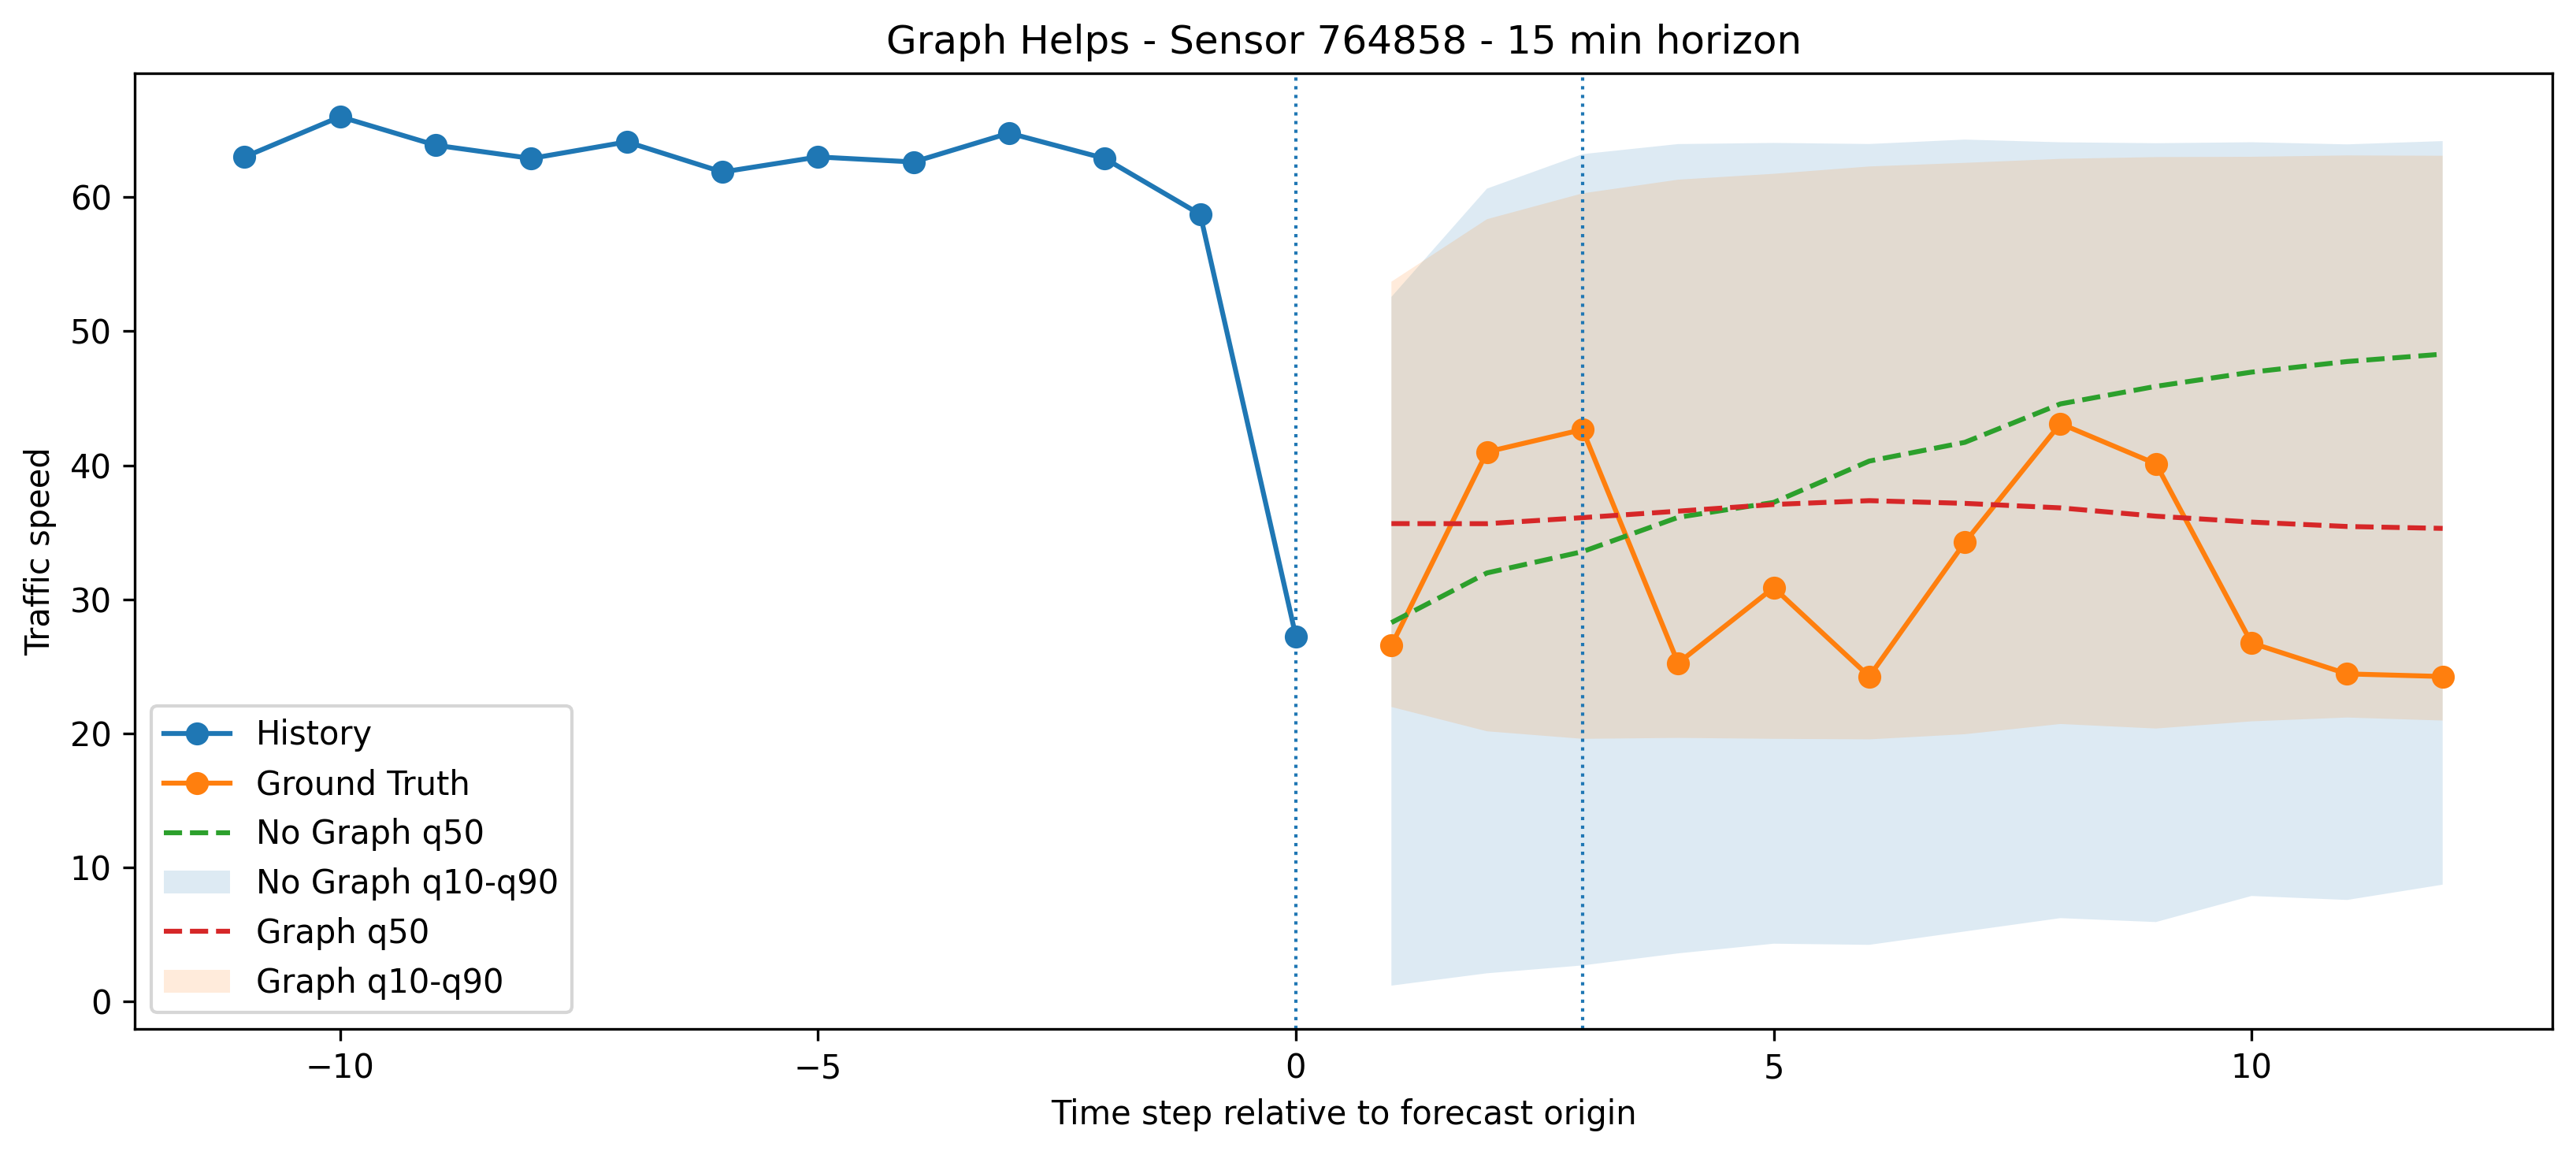
\includegraphics[width=\linewidth]{img/graph_impact_analysis/graph_helps_h3_sensor_764858}
    \end{minipage}
    \hfill
    \begin{minipage}[b]{0.8\linewidth}
        \centering
        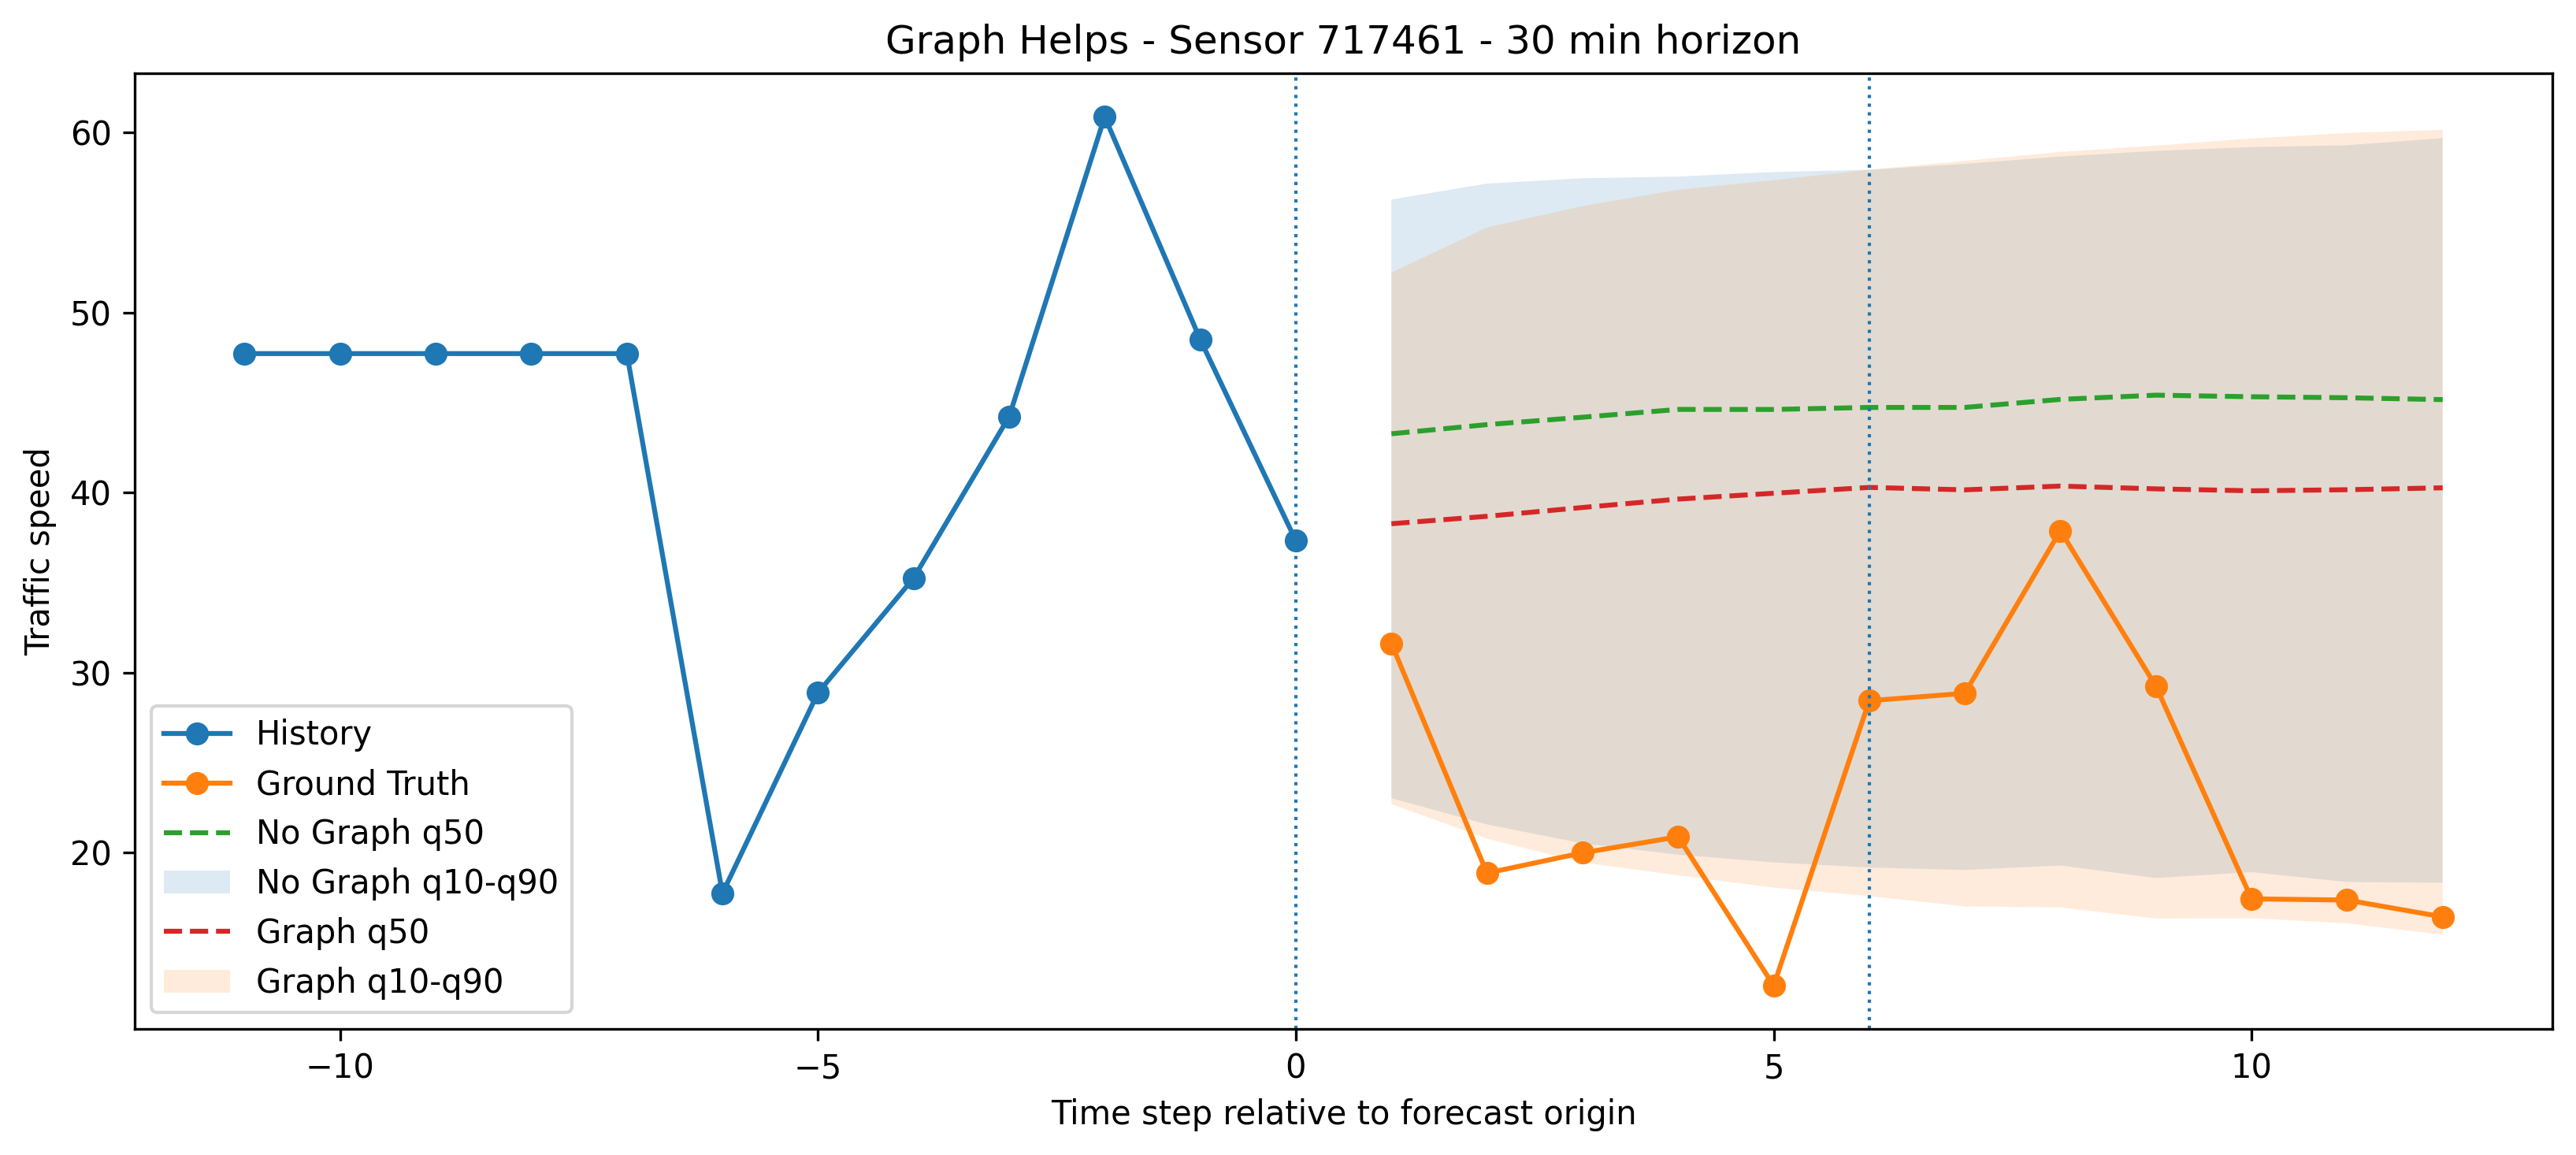
\includegraphics[width=\linewidth]{img/graph_impact_analysis/graph_helps_h6_sensor_717461}
    \end{minipage}
    \hfill
    \begin{minipage}[b]{0.8\linewidth}
        \centering
        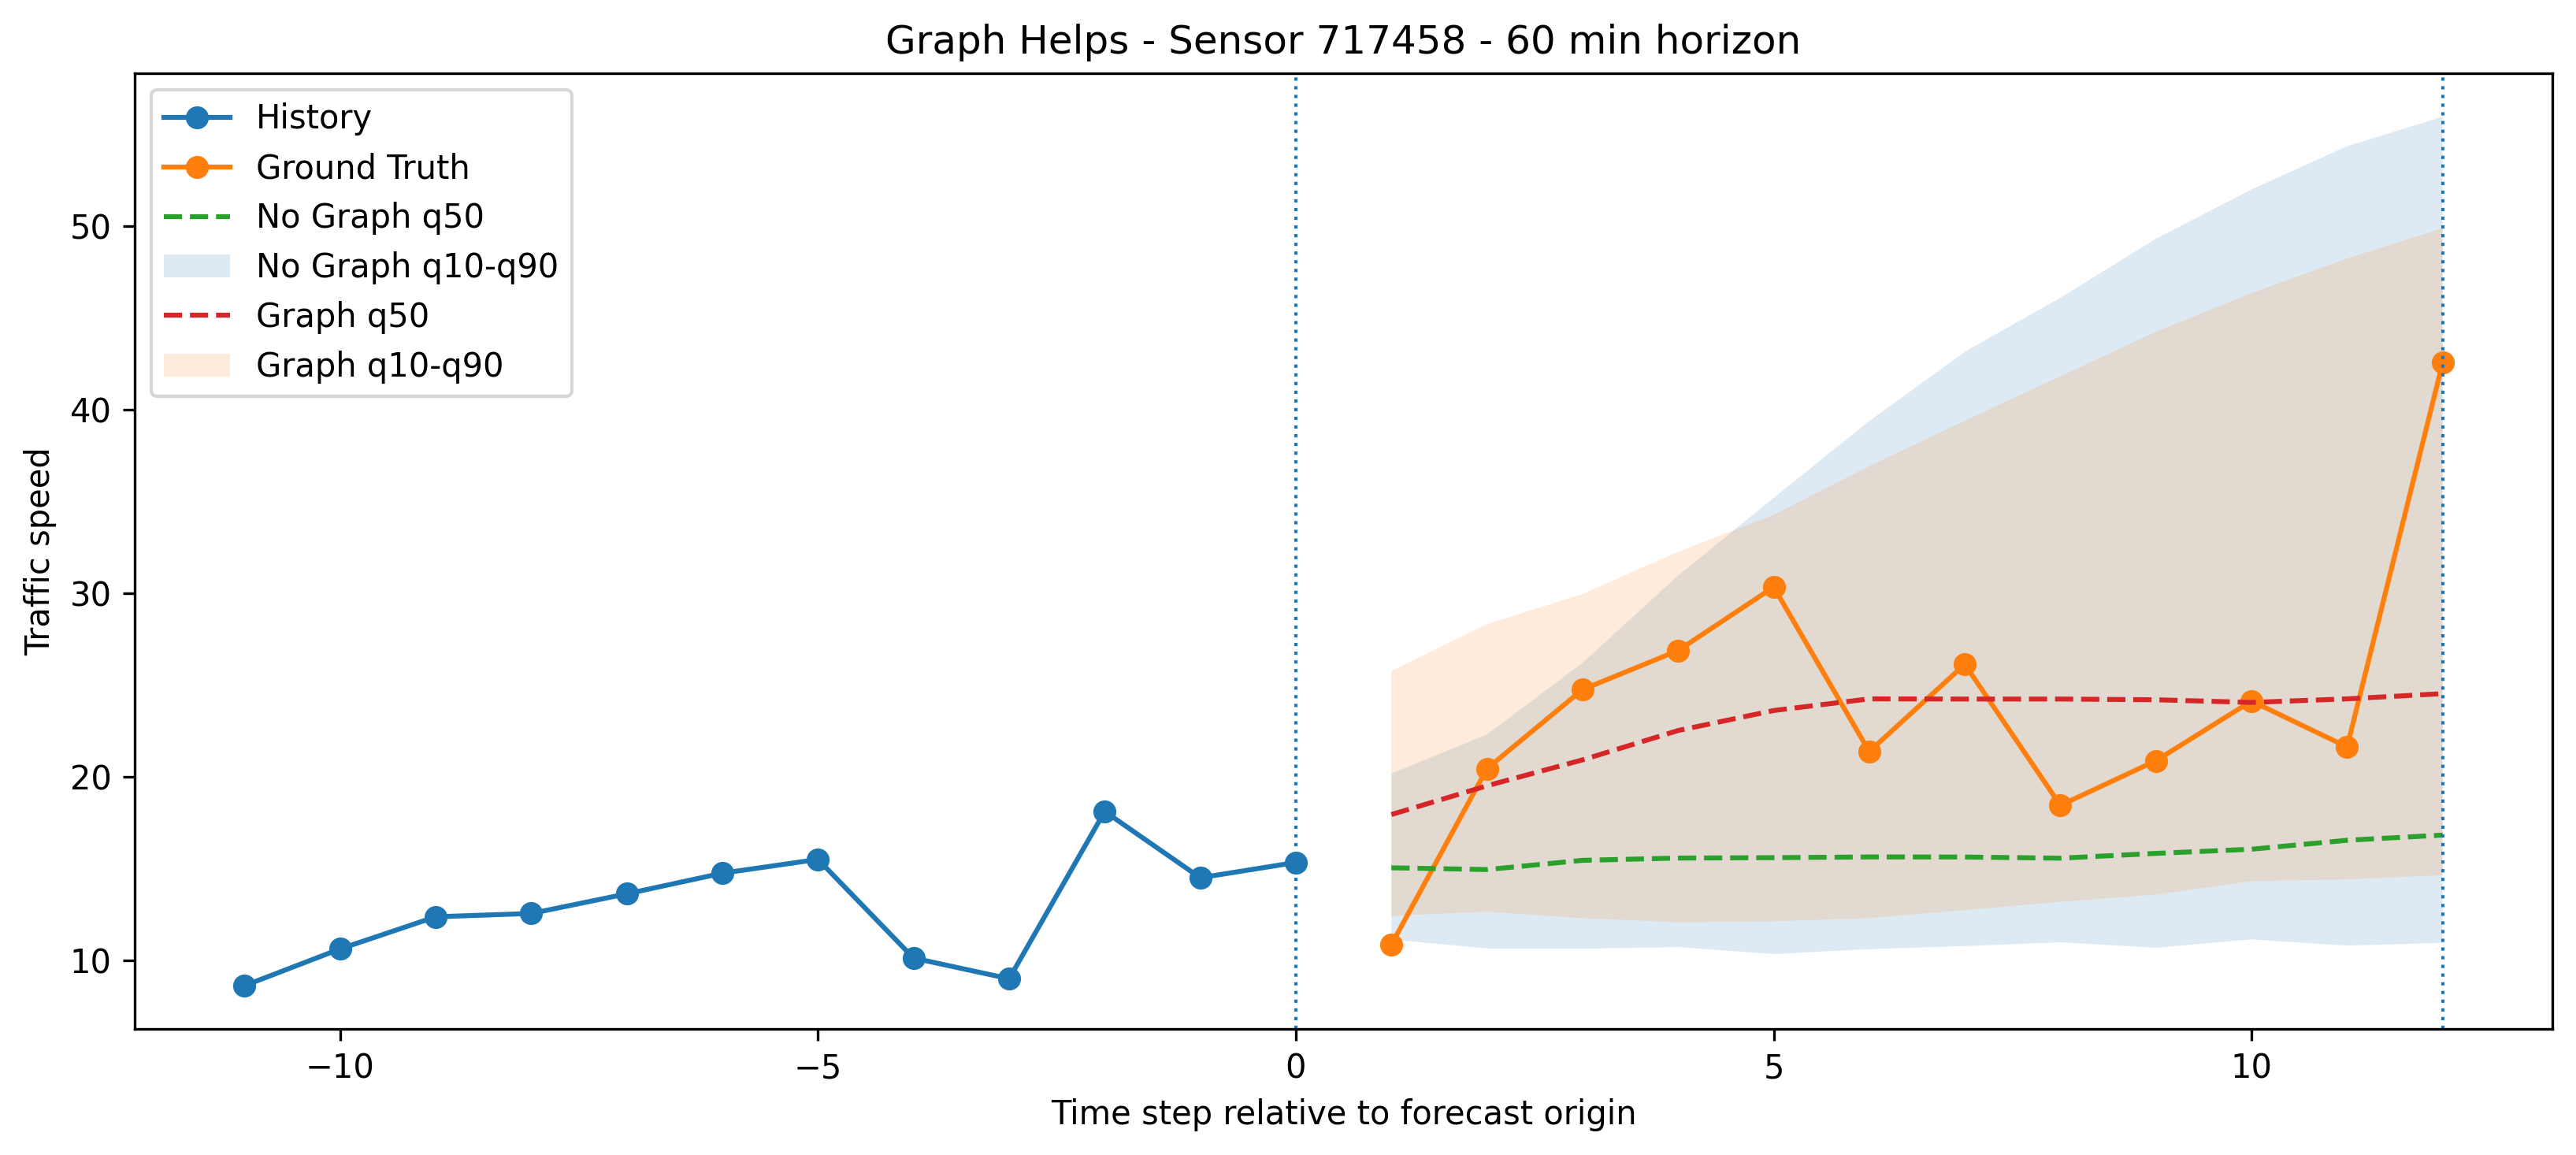
\includegraphics[width=\linewidth]{img/graph_impact_analysis/graph_helps_h12_sensor_717458}
    \end{minipage}

    \caption{Representative forecasting examples in which the Graph-Temporal
    model improves over the Temporal GRU at the 15-minute (left), 30-minute
    (center), and 60-minute (right) forecasting horizons.}
    \label{fig:graph_help_examples}
\end{figure}


Figure~\ref{fig:graph_hurt_examples} instead reports representative cases in
which graph message passing increases the forecasting error. These examples
are particularly useful because they show that neighboring information is
not always informative for the future evolution of a given sensor. The
presence of such cases motivates a more detailed investigation of whether the
benefit of graph message passing can be related to the local graph structure.

\begin{figure}[t]
    \centering

    \begin{minipage}[b]{0.8\linewidth}
        \centering
        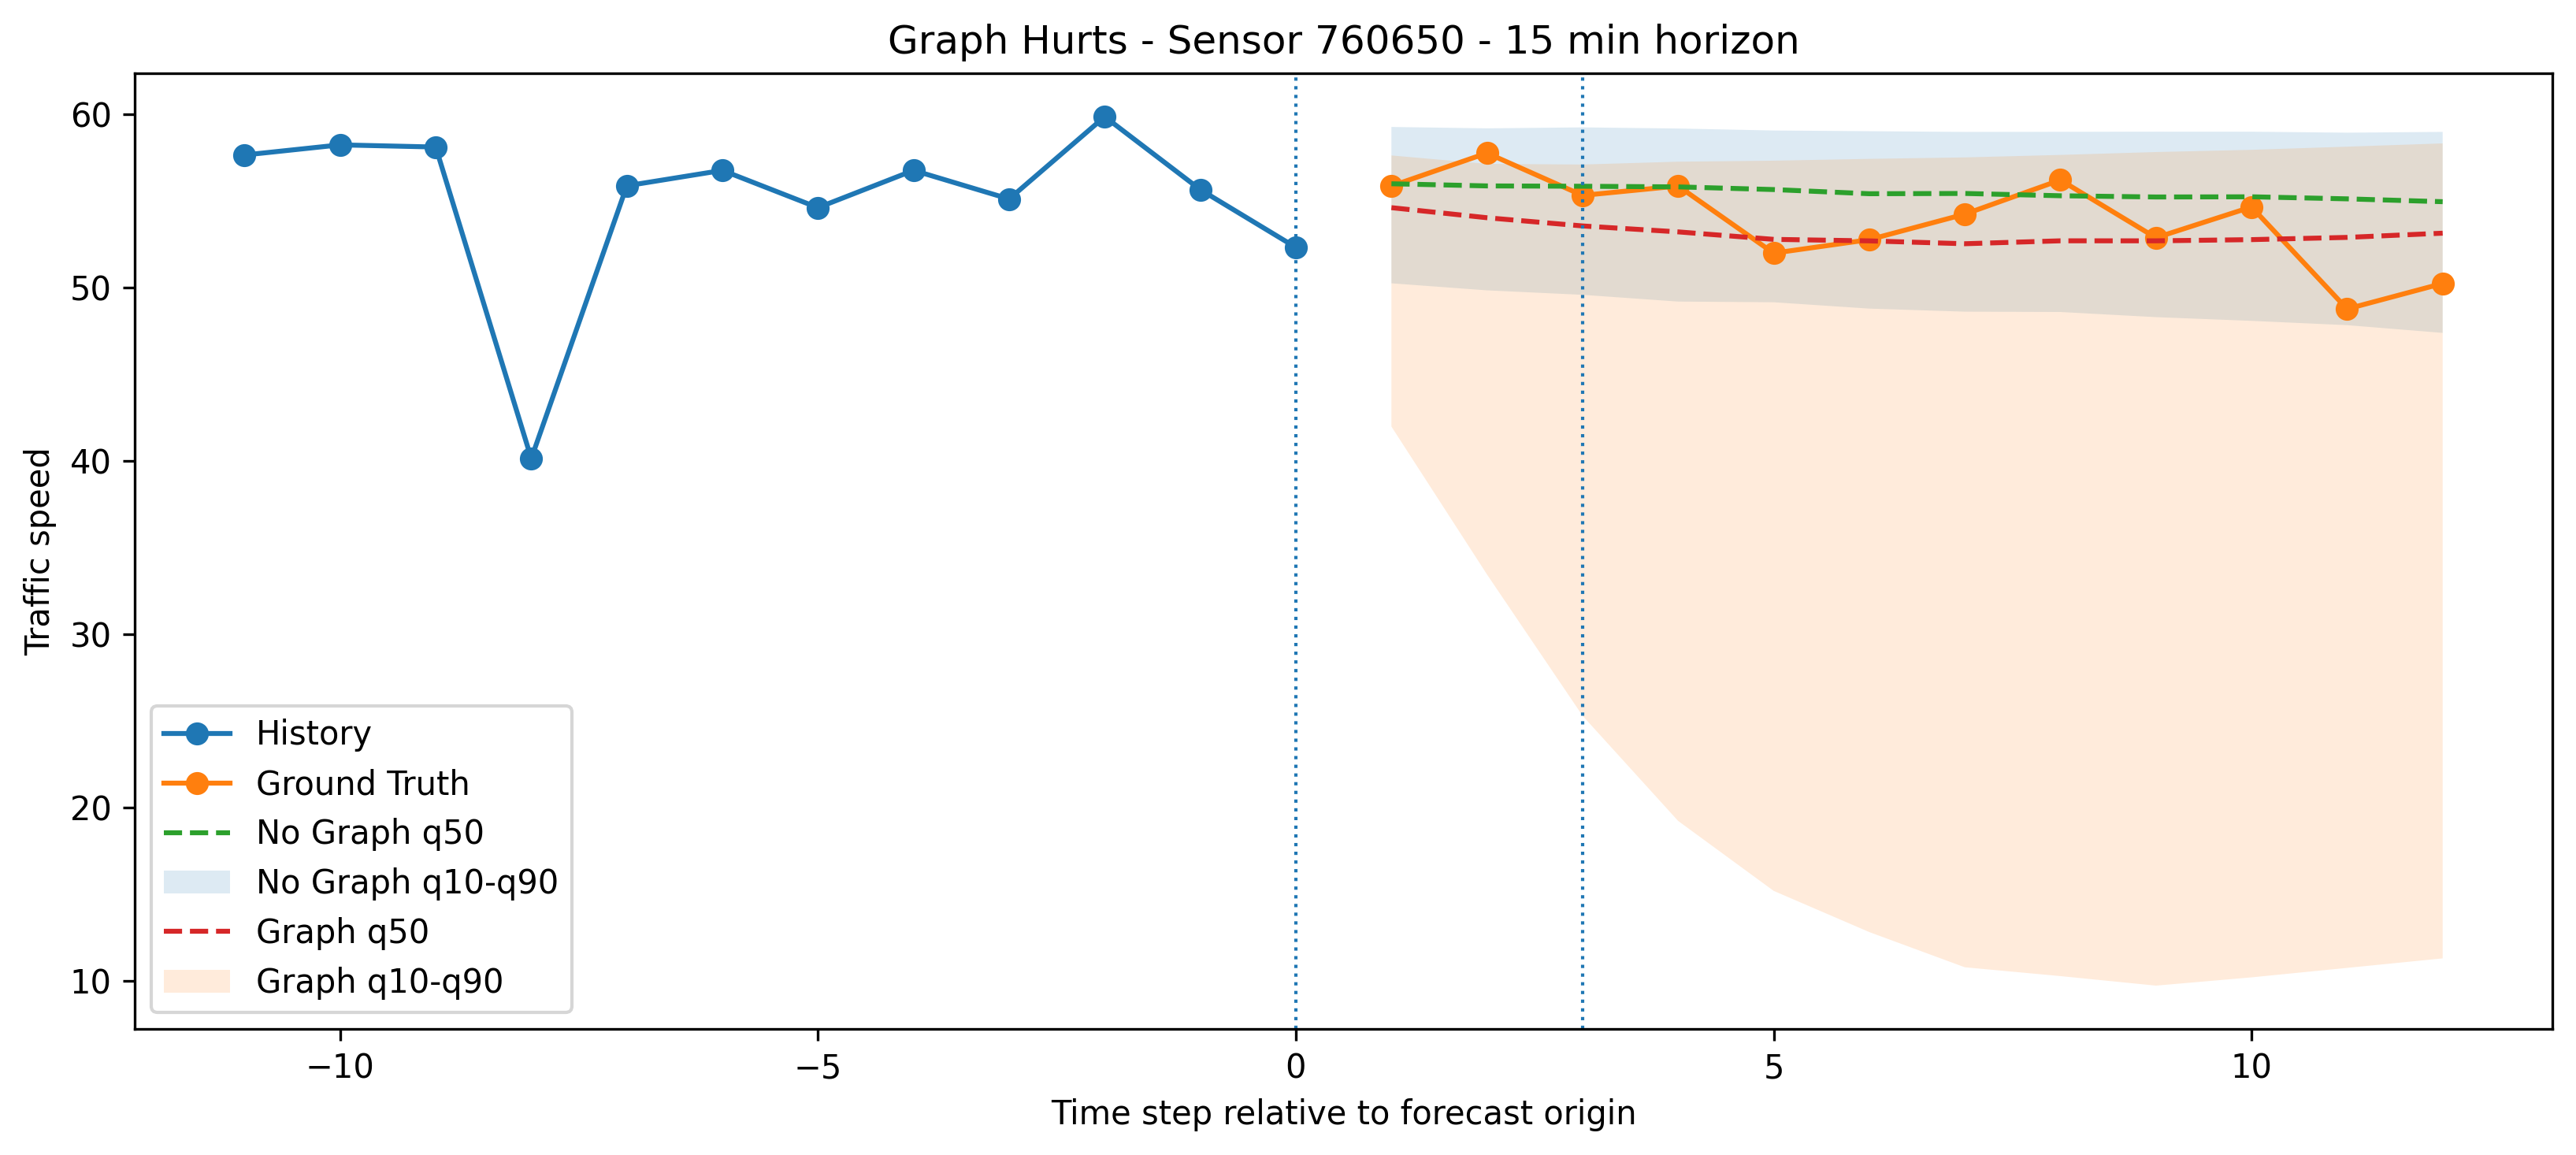
\includegraphics[width=\linewidth]{img/graph_impact_analysis/graph_hurts_h3_sensor_760650}
    \end{minipage}
    \hfill
    \begin{minipage}[b]{0.8\linewidth}
        \centering
        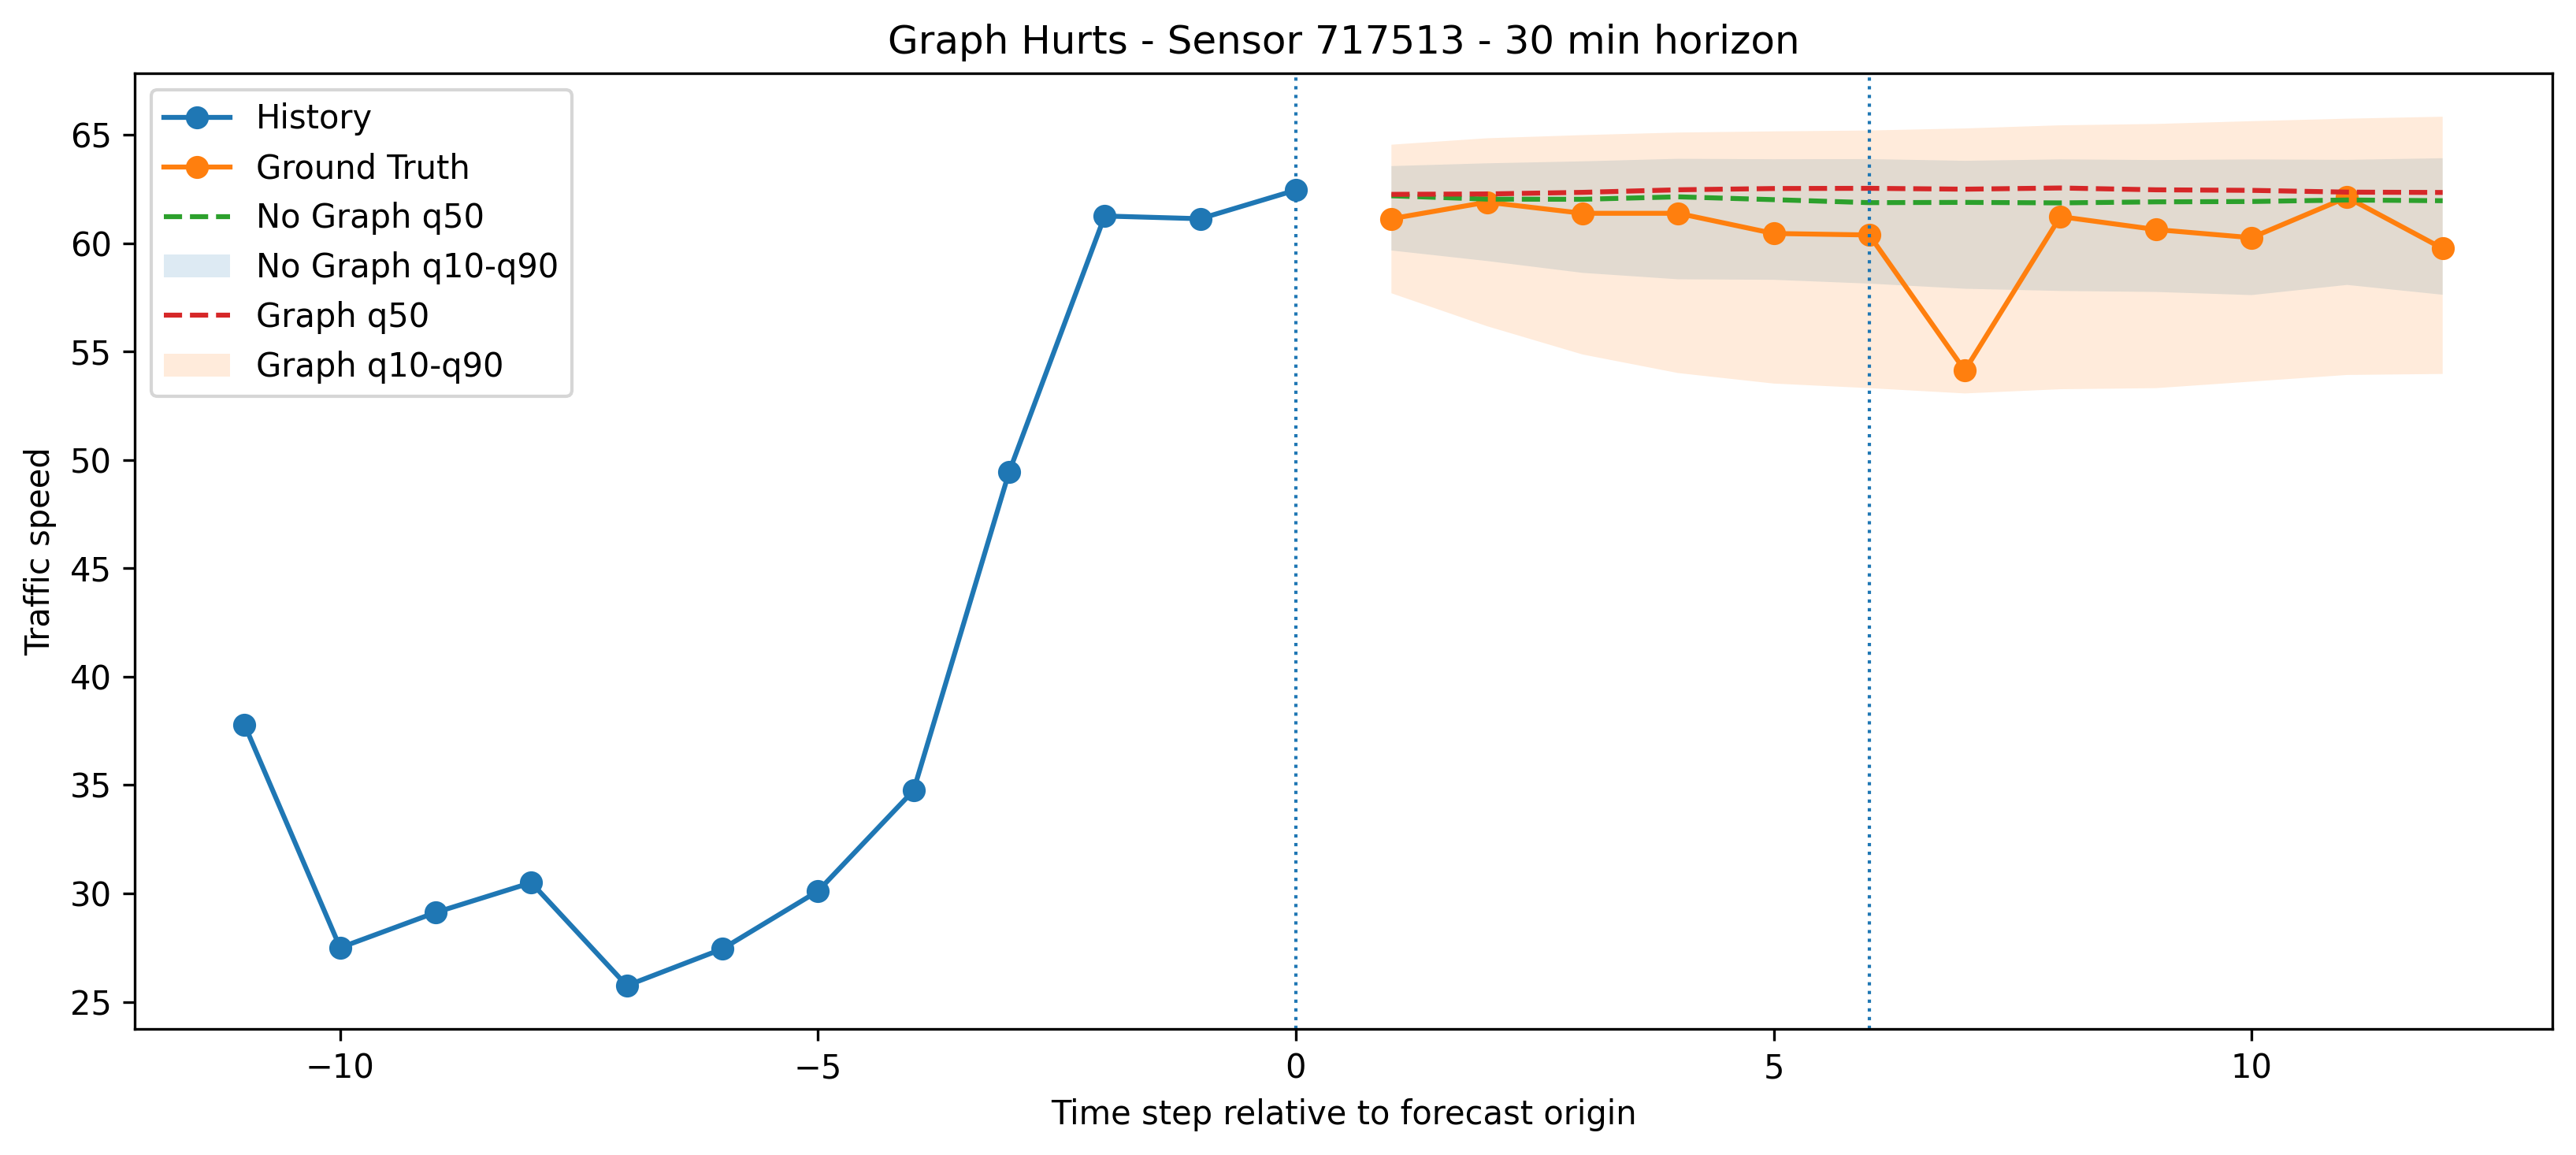
\includegraphics[width=\linewidth]{img/graph_impact_analysis/graph_hurts_h6_sensor_717513}
    \end{minipage}
    \hfill
    \begin{minipage}[b]{0.8\linewidth}
        \centering
        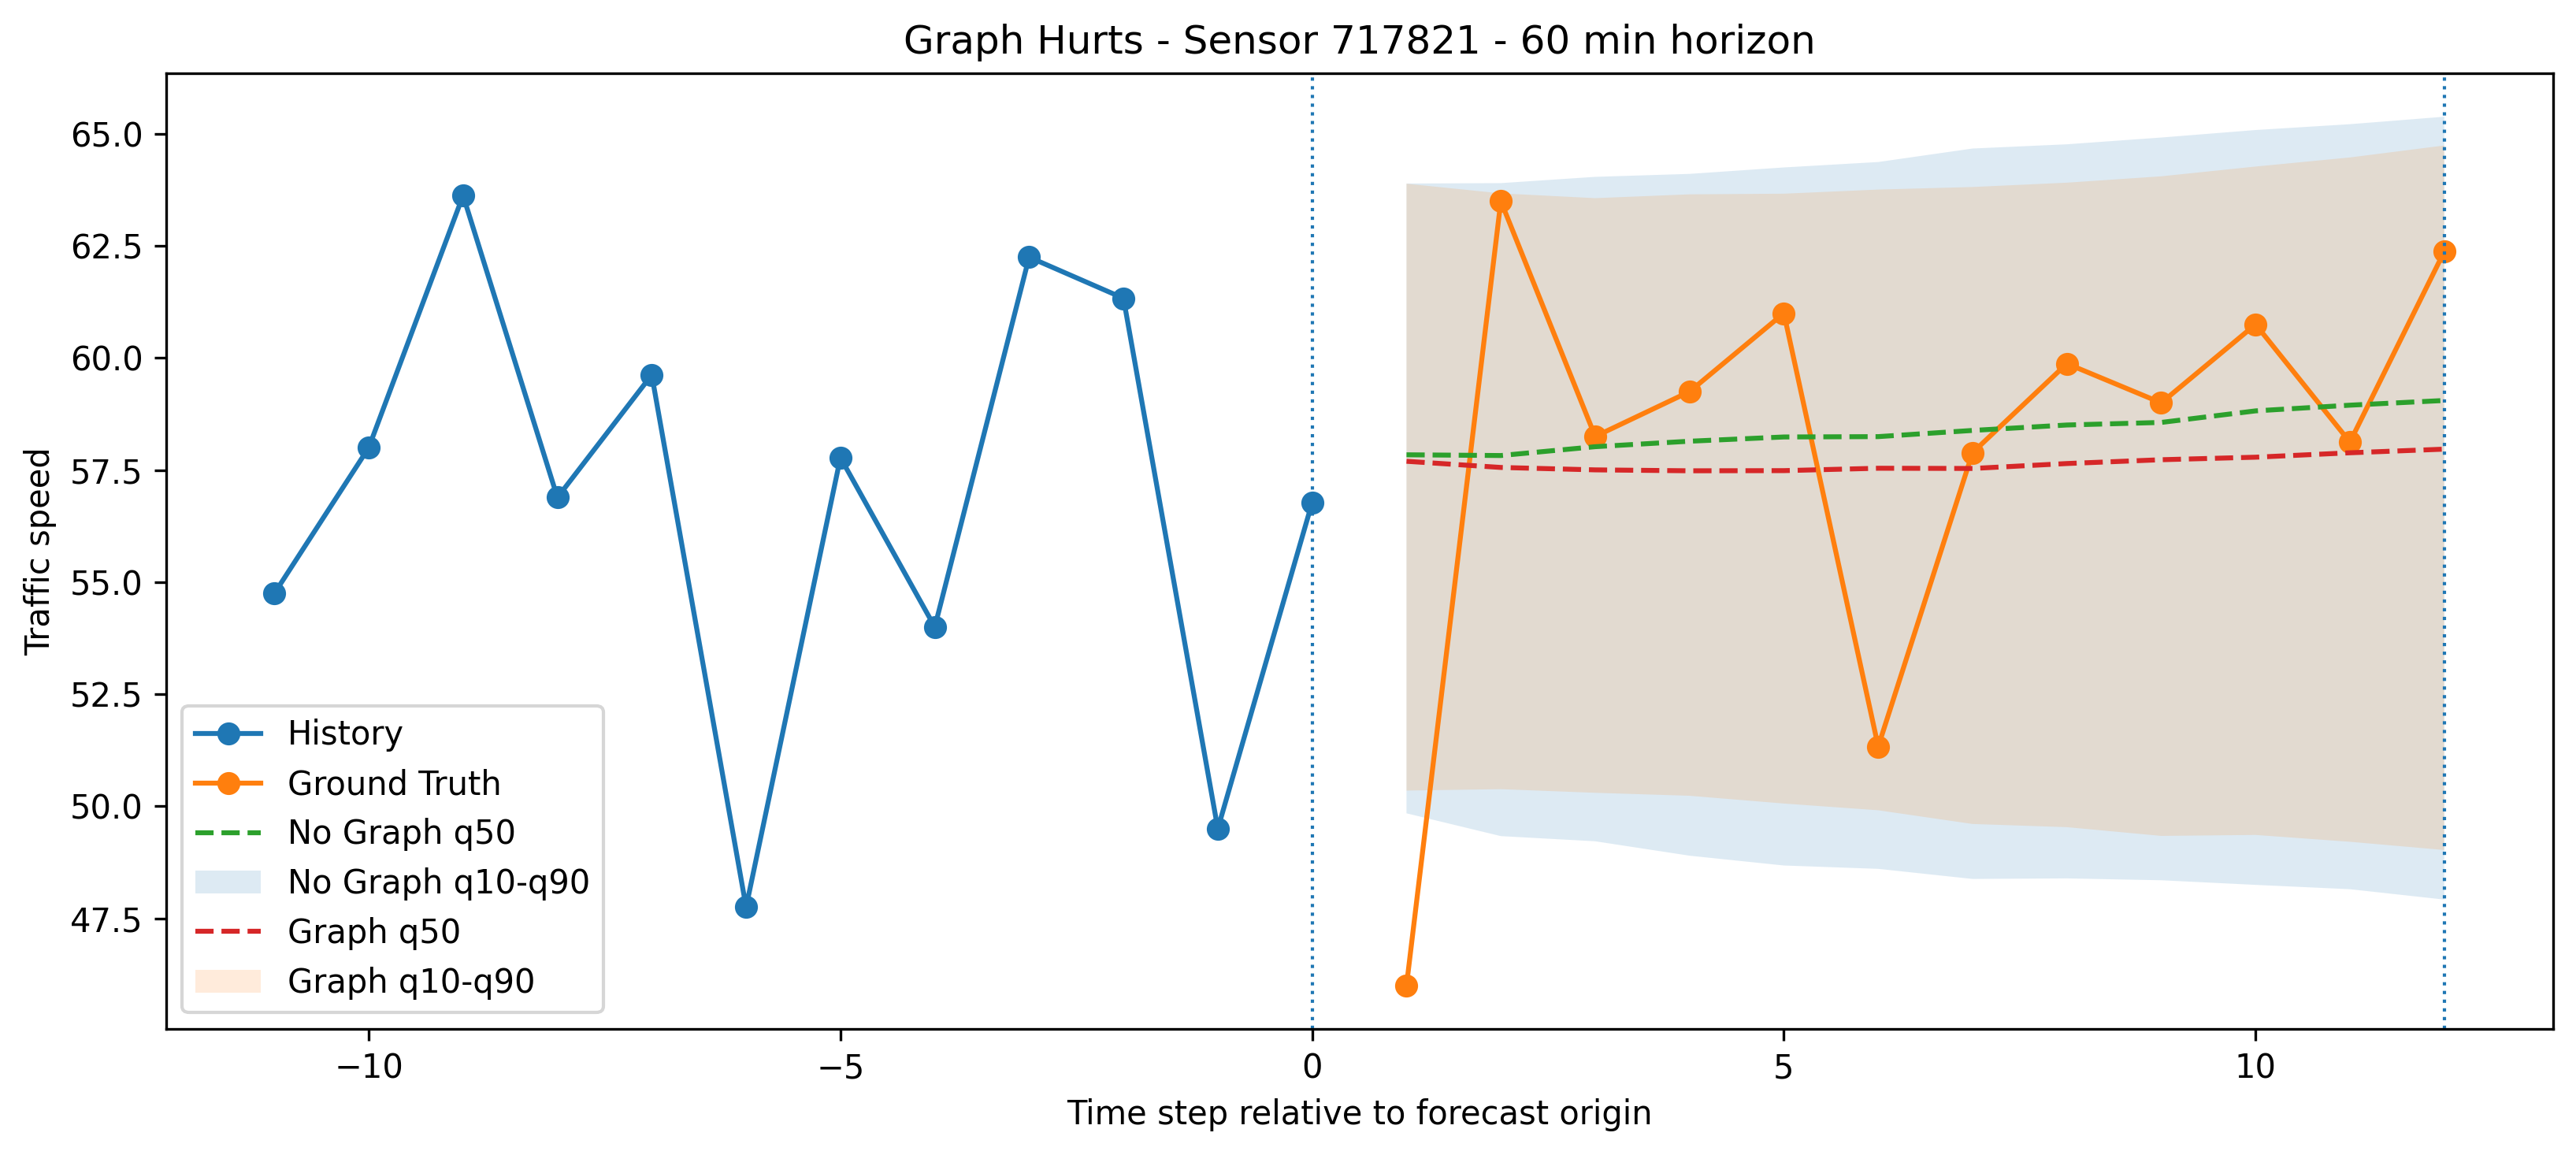
\includegraphics[width=\linewidth]{img/graph_impact_analysis/graph_hurts_h12_sensor_717821}
    \end{minipage}

    \caption{Representative forecasting examples in which the Graph-Temporal
model performs worse than the Temporal GRU at the 15-minute (left), 30-minute
(center), and 60-minute (right) forecasting horizons.}
    \label{fig:graph_hurt_examples}
\end{figure}

Overall, these examples confirm that the effect of graph message passing is
sensor- and time-dependent. Although spatial information improves forecasting
accuracy for the large majority of sensors, it can occasionally introduce
information that does not improve the local prediction. This observation is
consistent with the small subset of sensors for which the Temporal GRU
achieves lower MAE.

\subsection{Effect of Diffusion Depth}
\label{subsec:diffusion_depth}

The main Graph-Temporal model uses a diffusion depth of $K=2$, allowing each
diffusion layer to combine information from the current node and from nodes
reached through one and two-step propagation. To investigate whether a
larger spatial receptive field provides additional benefits, a variant with
$K=3$ was trained while keeping the remaining model configuration unchanged.

Table~\ref{tab:diffusion_depth} compares the test performance of the two
configurations. Increasing the diffusion depth produces a small but consistent
reduction in MAE. However, the same behavior
is not observed for RMSE since $K=3$ model obtains slightly higher RMSE at all
three horizons. Therefore, the additional diffusion step
slightly improves the average absolute error but does not improve the model's
sensitivity to larger forecasting errors.


\begin{table}[t]
    \centering
    \caption{Test performance of the Graph-Temporal model with diffusion
    depths $K=2$ and $K=3$.}
    \label{tab:diffusion_depth}
    \resizebox{\linewidth}{!}{
    \begin{tabular}{ccrrrrr}
        \toprule
        $K$ & Horizon &
        MAE & RMSE & Coverage (\%) & Interval Width & Crossing (\%) \\
        \midrule
        2 & 15 min & 2.901 & 5.511 & 78.44 & 8.929  & 0.031 \\
        2 & 30 min & 3.442 & 6.758 & 78.22 & 10.485 & 0.029 \\
        2 & 60 min & 4.244 & 8.378 & 78.13 & 12.470 & 0.048 \\
        \midrule
        3 & 15 min & 2.888 & 5.533 & 78.84 & 8.723  & 0.028 \\
        3 & 30 min & 3.424 & 6.799 & 77.87 & 9.948  & 0.034 \\
        3 & 60 min & 4.203 & 8.384 & 77.50 & 11.781 & 0.055 \\
        \bottomrule
    \end{tabular}}
\end{table}


\begin{figure}[t]
    \centering

    % First row: point forecasting metrics
    \begin{minipage}[b]{0.48\linewidth}
        \centering
        
\includegraphics[width=\linewidth]{img/graph_temporal/variant_comparison/mae_graph_temporal_variant_comparison}
    \end{minipage}
    \hfill
    \begin{minipage}[b]{0.48\linewidth}
        \centering
        
\includegraphics[width=\linewidth]{img/graph_temporal/variant_comparison/rmse_graph_temporal_variant_comparison}
    \end{minipage}

    \vspace{0.4cm}

    % Second row: probabilistic metrics
    \begin{minipage}[b]{0.48\linewidth}
        \centering
        
\includegraphics[width=\linewidth]{img/graph_temporal/variant_comparison//coverage_graph_temporal_variant_comparison}
    \end{minipage}
    \hfill
    \begin{minipage}[b]{0.48\linewidth}
        \centering
        
\includegraphics[width=\linewidth]{img/graph_temporal/variant_comparison/interval_width_graph_temporal_variant_comparison}
    \end{minipage}

    \caption{Comparison of the Graph-Temporal model with diffusion depths
    $K=2$ and $K=3$. The top row reports point forecasting performance in
    terms of MAE (left) and RMSE (right), while the bottom row reports
    empirical coverage (left) and prediction interval width (right) across
    the three forecasting horizons.}
    \label{fig:diffusion_depth_comparison}
\end{figure}

The comparison is also illustrated in
Figure~\ref{fig:diffusion_depth_comparison}. The effect of the additional
diffusion step is particularly visible in the probabilistic forecasts.
The $K=3$ model produces narrower prediction intervals at every horizon.
At the shortest horizon, this increased sharpness is accompanied by a small
improvement in coverage. At the longer forecasting horizons, however, the
sharper intervals obtained with $K=3$ come at the cost of increased
undercoverage. Quantile crossing remains negligible for both configurations.

The two configurations also exhibit different computational behavior. The
$K=2$ model was trained for 106 epochs, whereas the $K=3$ variant stopped
after 85 epochs. Despite requiring fewer epochs, the additional diffusion
step increases the computational cost of each epoch: the average training
time rises from approximately 19.3 seconds per epoch for $K=2$ to 22.0
seconds for $K=3$, an increase of about 14\%. The total training times are
approximately 34.0 and 31.1 minutes, respectively, with the lower total
training time of $K=3$ resulting from earlier stopping rather than lower
per-epoch computational complexity.

Overall, increasing the diffusion depth from $K=2$ to $K=3$ provides only
modest improvements in MAE and median Pinball Loss, while slightly increasing
RMSE and reducing coverage at the longer horizons. It also increases the
computational cost of each training epoch. For these reasons, $K=2$ was
retained for the main Graph-Temporal model, providing a more balanced
trade-off between forecasting accuracy, probabilistic reliability, and
computational complexity.

\subsection{Graph Ablation: Weighted vs. Binary Adjacency}
\label{subsec:weighted_binary}

The previous experiments use the original weighted adjacency matrix provided
with METR-LA. To investigate whether the edge weights contribute to the
forecasting performance or whether the graph connectivity alone is sufficient,
an ablation experiment was performed by replacing every non-zero edge weight
with one. The resulting binary adjacency matrix preserves the original graph
topology but removes information about the relative strength of the
connections. As for the weighted graph, the binary adjacency matrix was
row-normalized before being used for diffusion message passing.

Table~\ref{tab:weighted_binary} compares the two graph representations on the
test set. The weighted graph consistently achieves lower point forecasting
errors and the difference becomes larger as the forecasting horizon increases.


\begin{table}[t]
    \centering
    \caption{Test performance of the Graph-Temporal model using the weighted
    and binary adjacency matrices.}
    \label{tab:weighted_binary}
    \resizebox{\linewidth}{!}{
    \begin{tabular}{llrrrr}
        \toprule
        Graph & Horizon & MAE & RMSE & Coverage (\%) & Interval Width \\
        \midrule
        Weighted
        & 15 min & 2.901 & 5.511 & 78.44 & 8.929 \\
        & 30 min & 3.442 & 6.758 & 78.22 & 10.485 \\
        & 60 min & 4.244 & 8.378 & 78.13 & 12.470 \\
        \midrule
        Binary
        & 15 min & 2.948 & 5.682 & 79.54 & 8.878 \\
        & 30 min & 3.543 & 7.033 & 78.80 & 10.424 \\
        & 60 min & 4.443 & 8.754 & 78.11 & 12.593 \\
        \bottomrule
    \end{tabular}}
\end{table}


\begin{figure}[t]
    \centering

    % First row: point forecasting metrics
    \begin{minipage}[b]{0.48\linewidth}
        \centering
        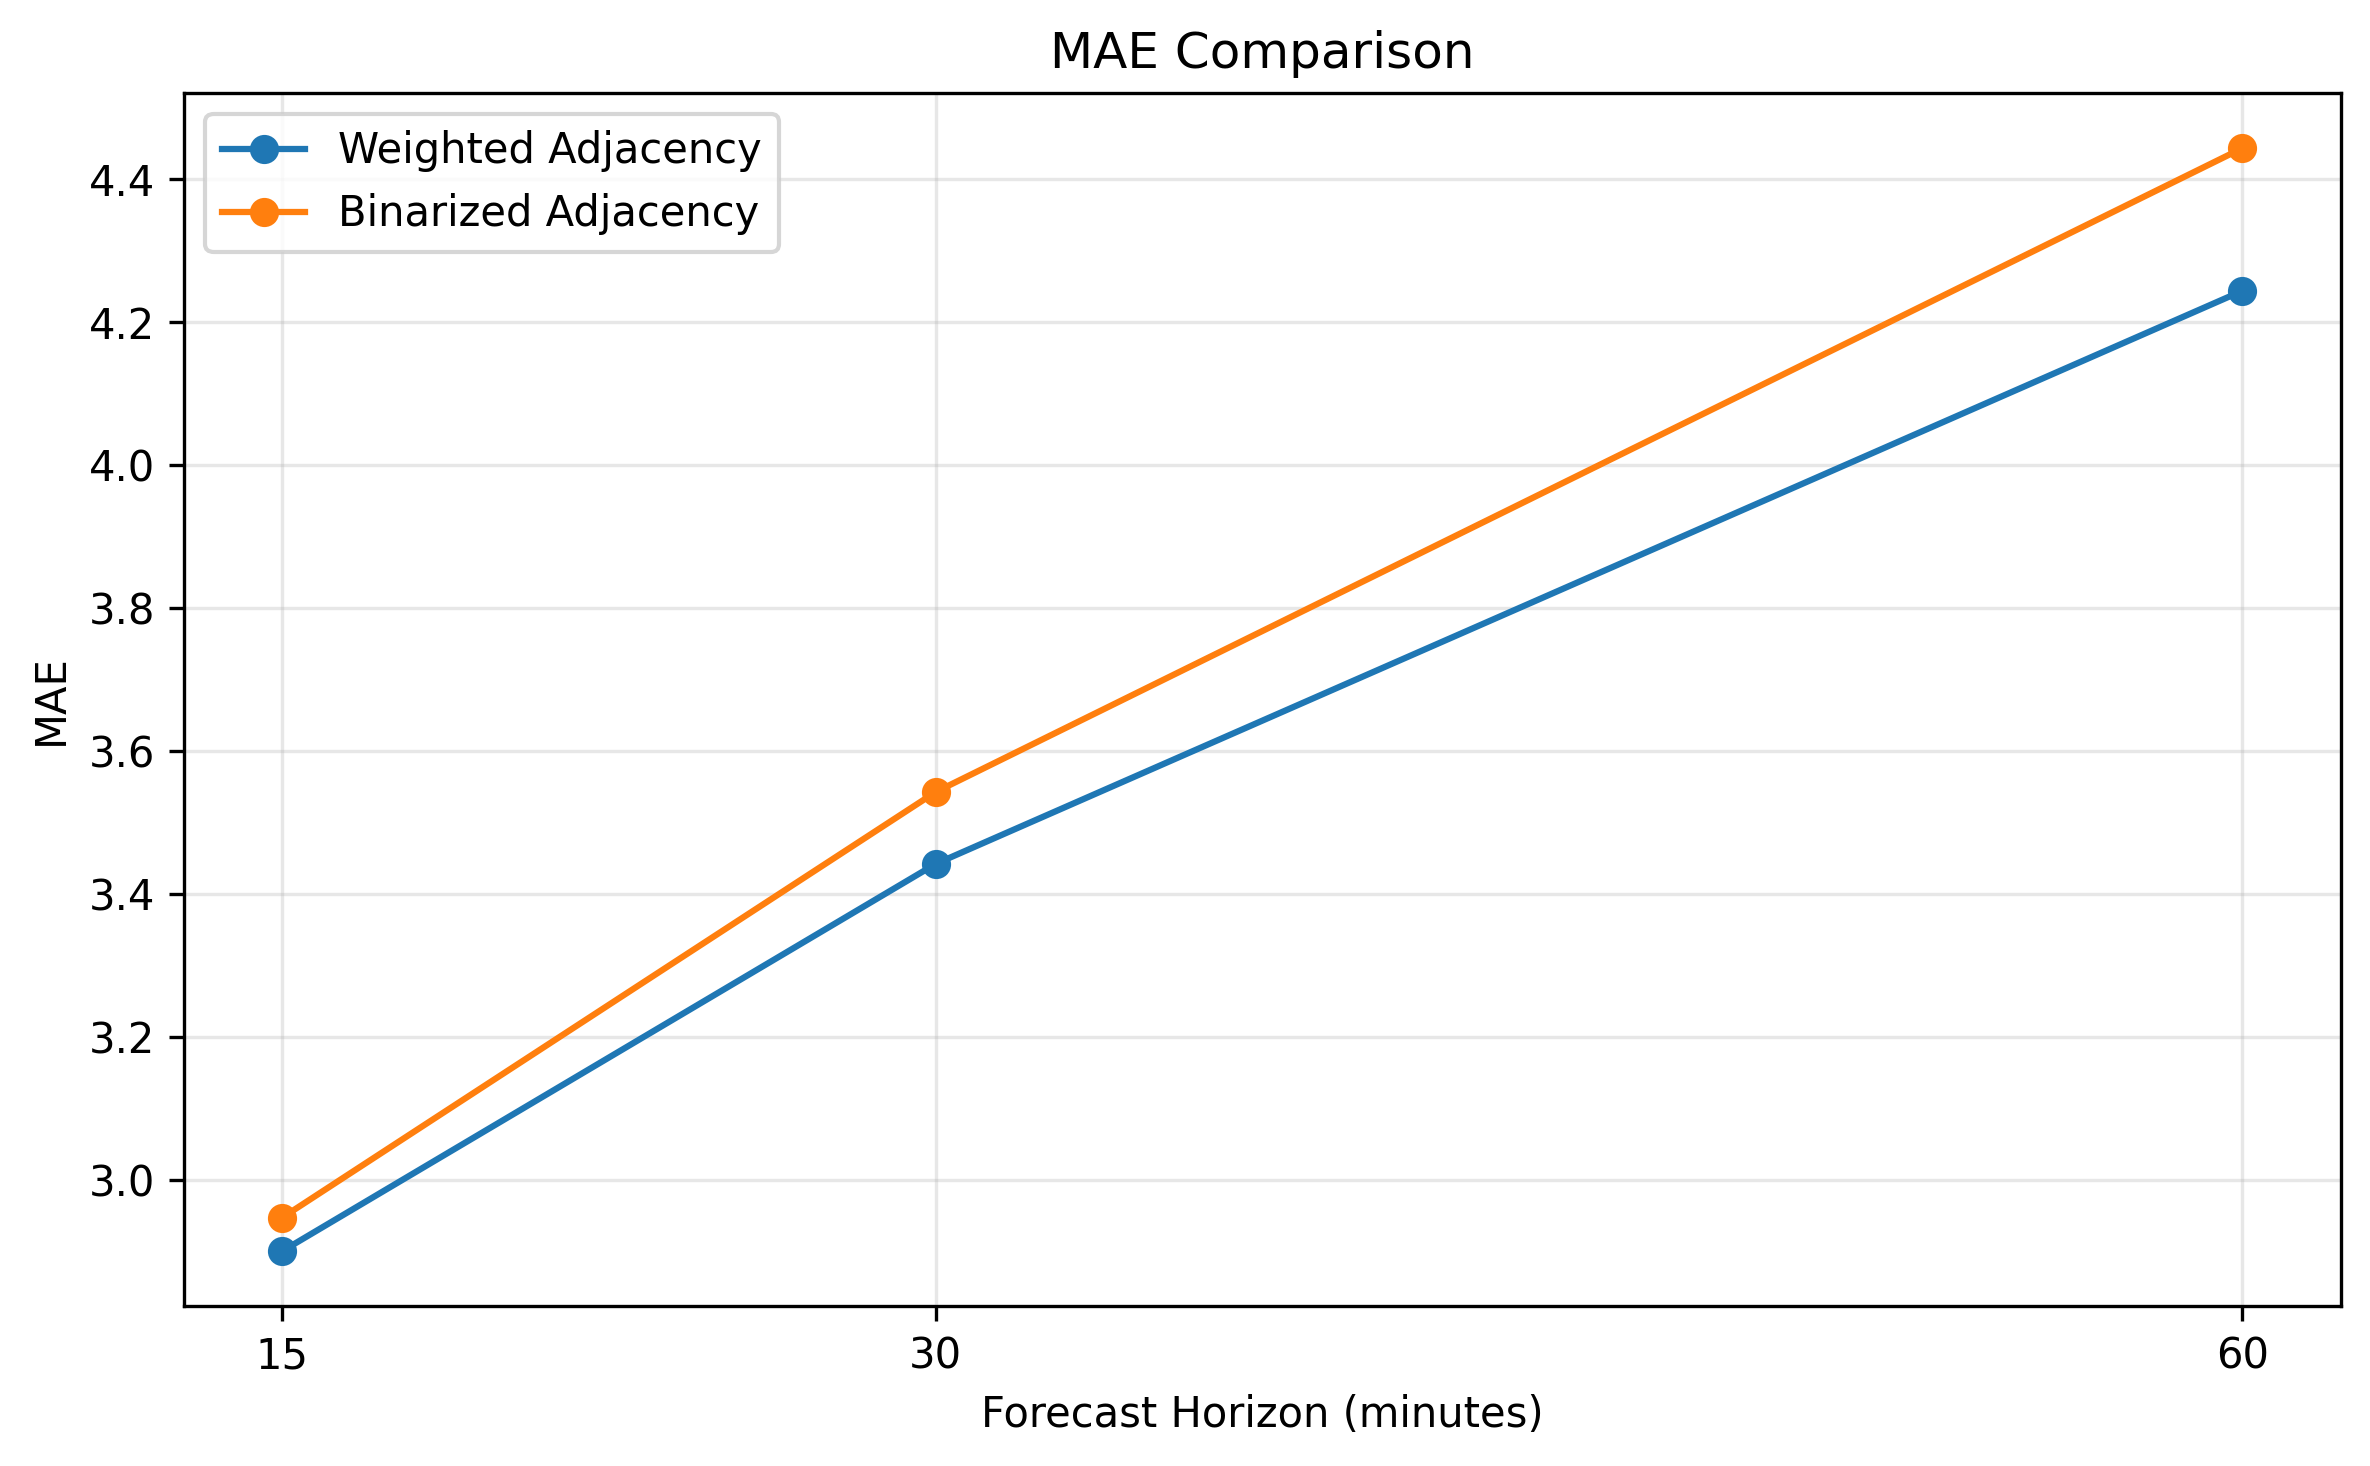
\includegraphics[width=\linewidth]{img/graph_temporal/ablation_comparison/mae_graph_temporal_variant_comparison}
    \end{minipage}
    \hfill
    \begin{minipage}[b]{0.48\linewidth}
        \centering
        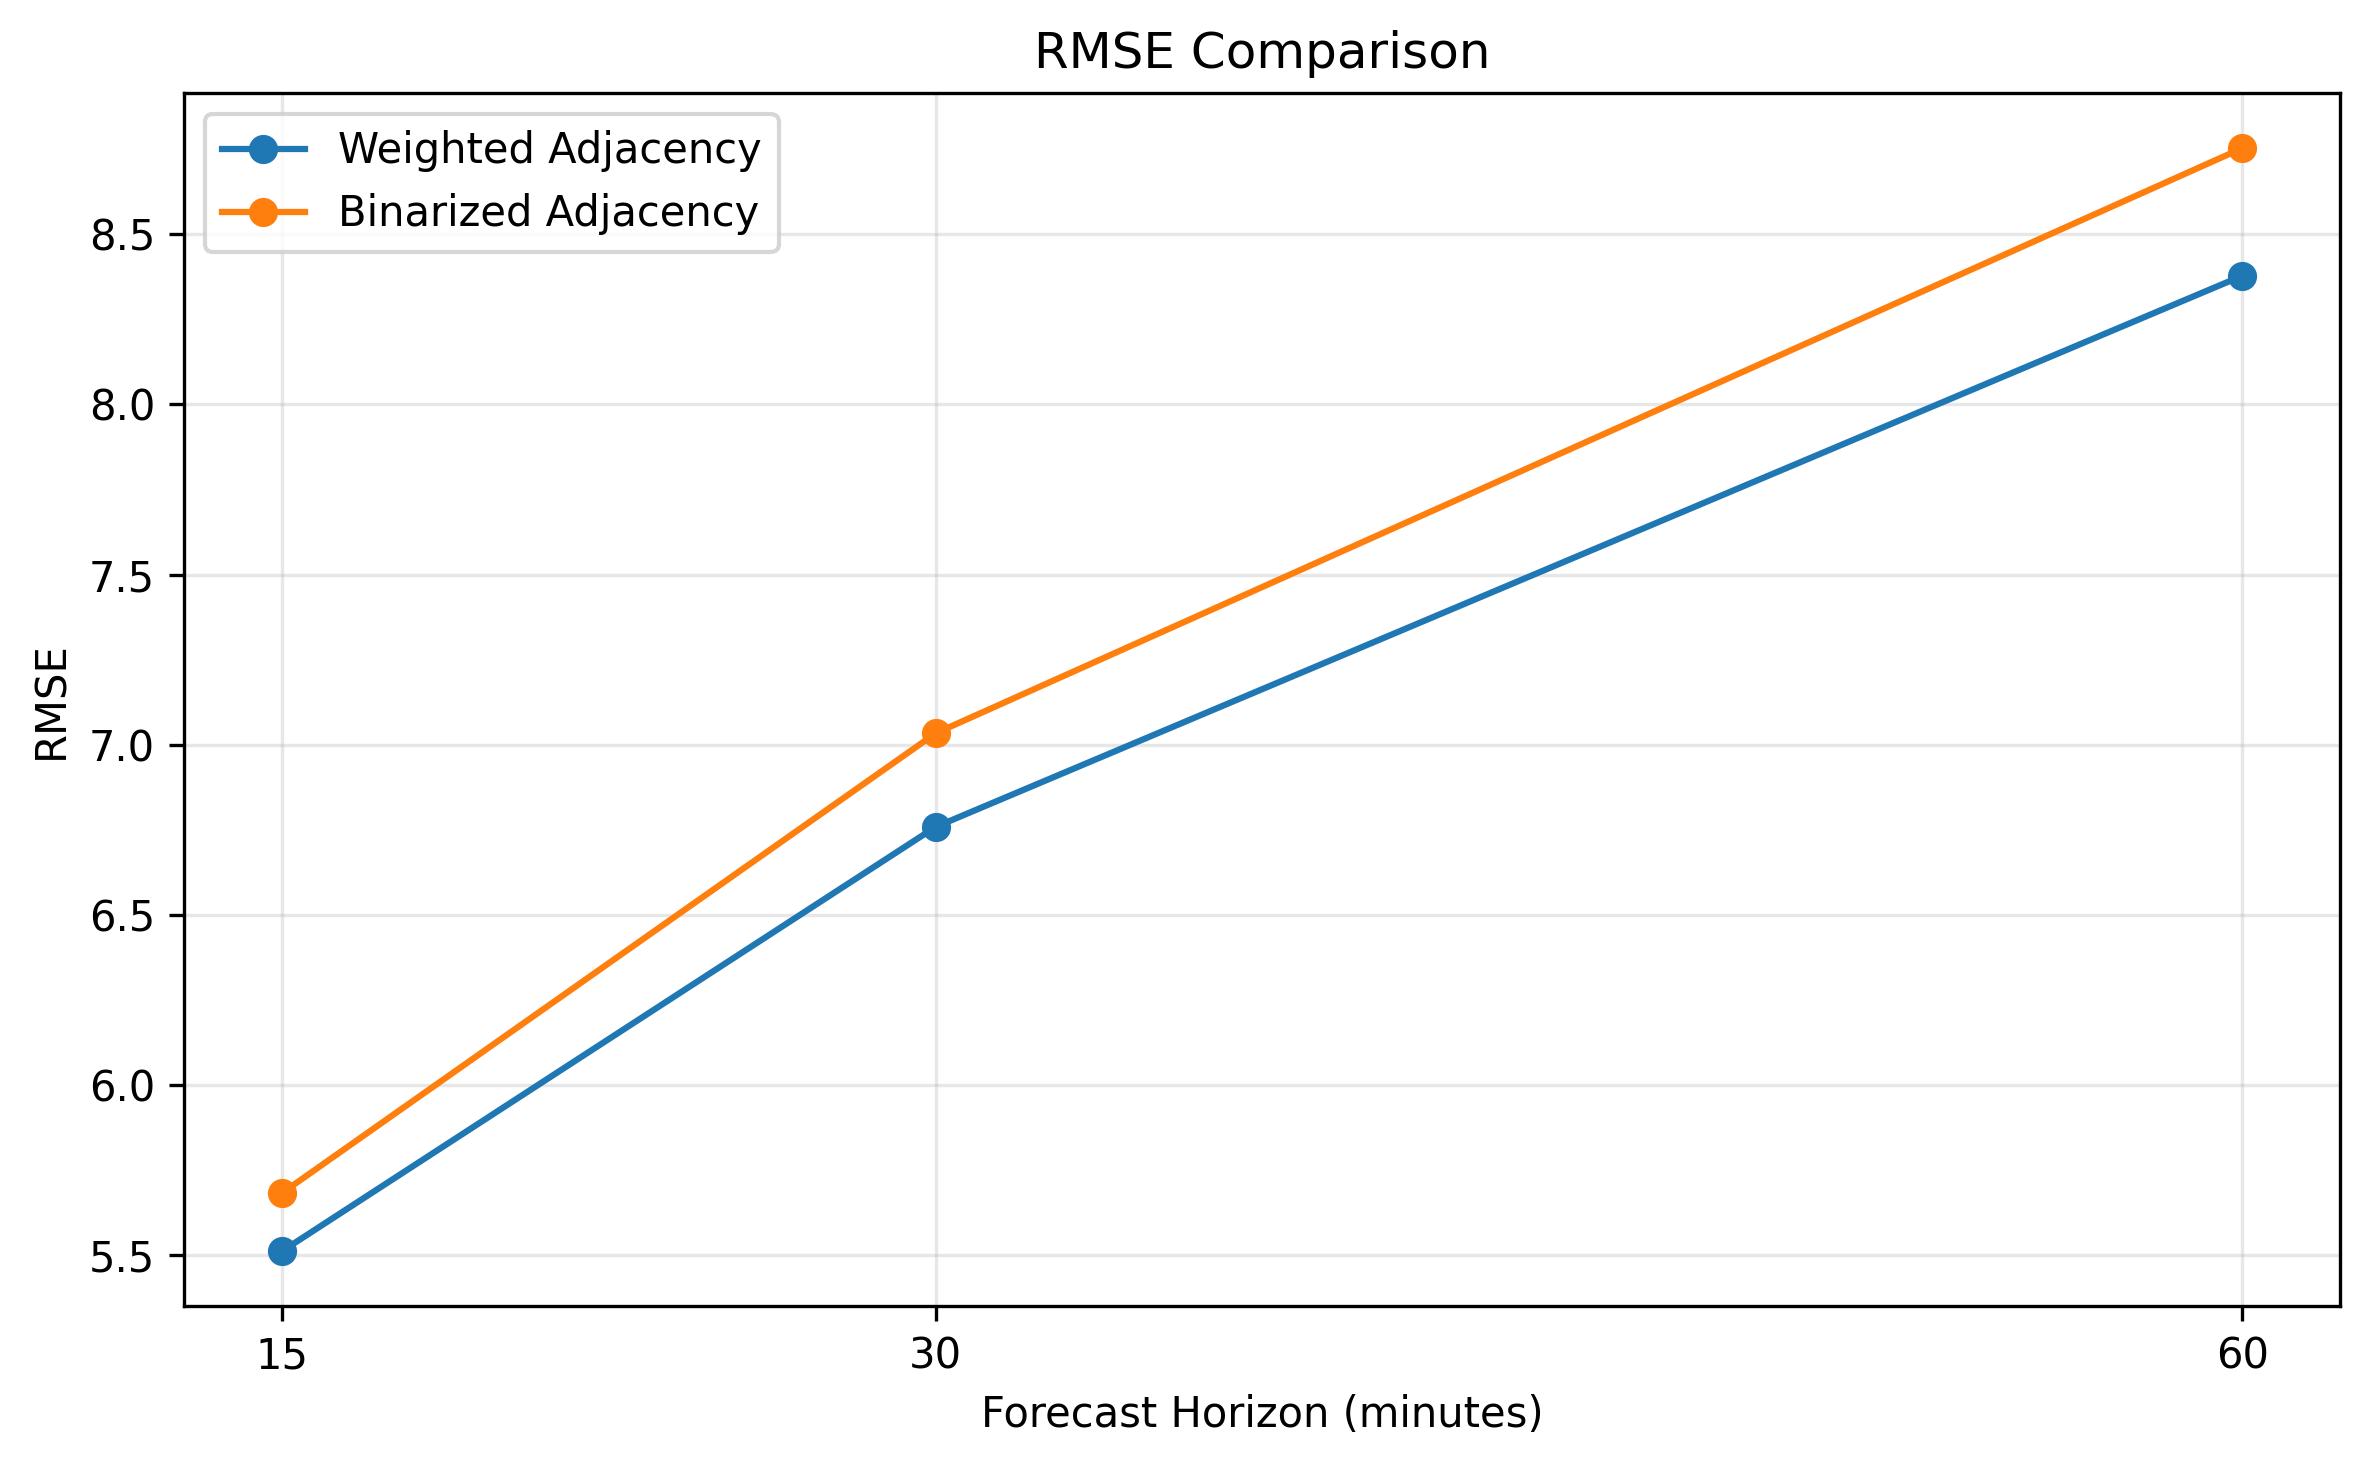
\includegraphics[width=\linewidth]{img/graph_temporal/ablation_comparison/rmse_graph_temporal_variant_comparison}
    \end{minipage}

    \vspace{0.4cm}

    % Second row: probabilistic metrics
    \begin{minipage}[b]{0.48\linewidth}
        \centering
        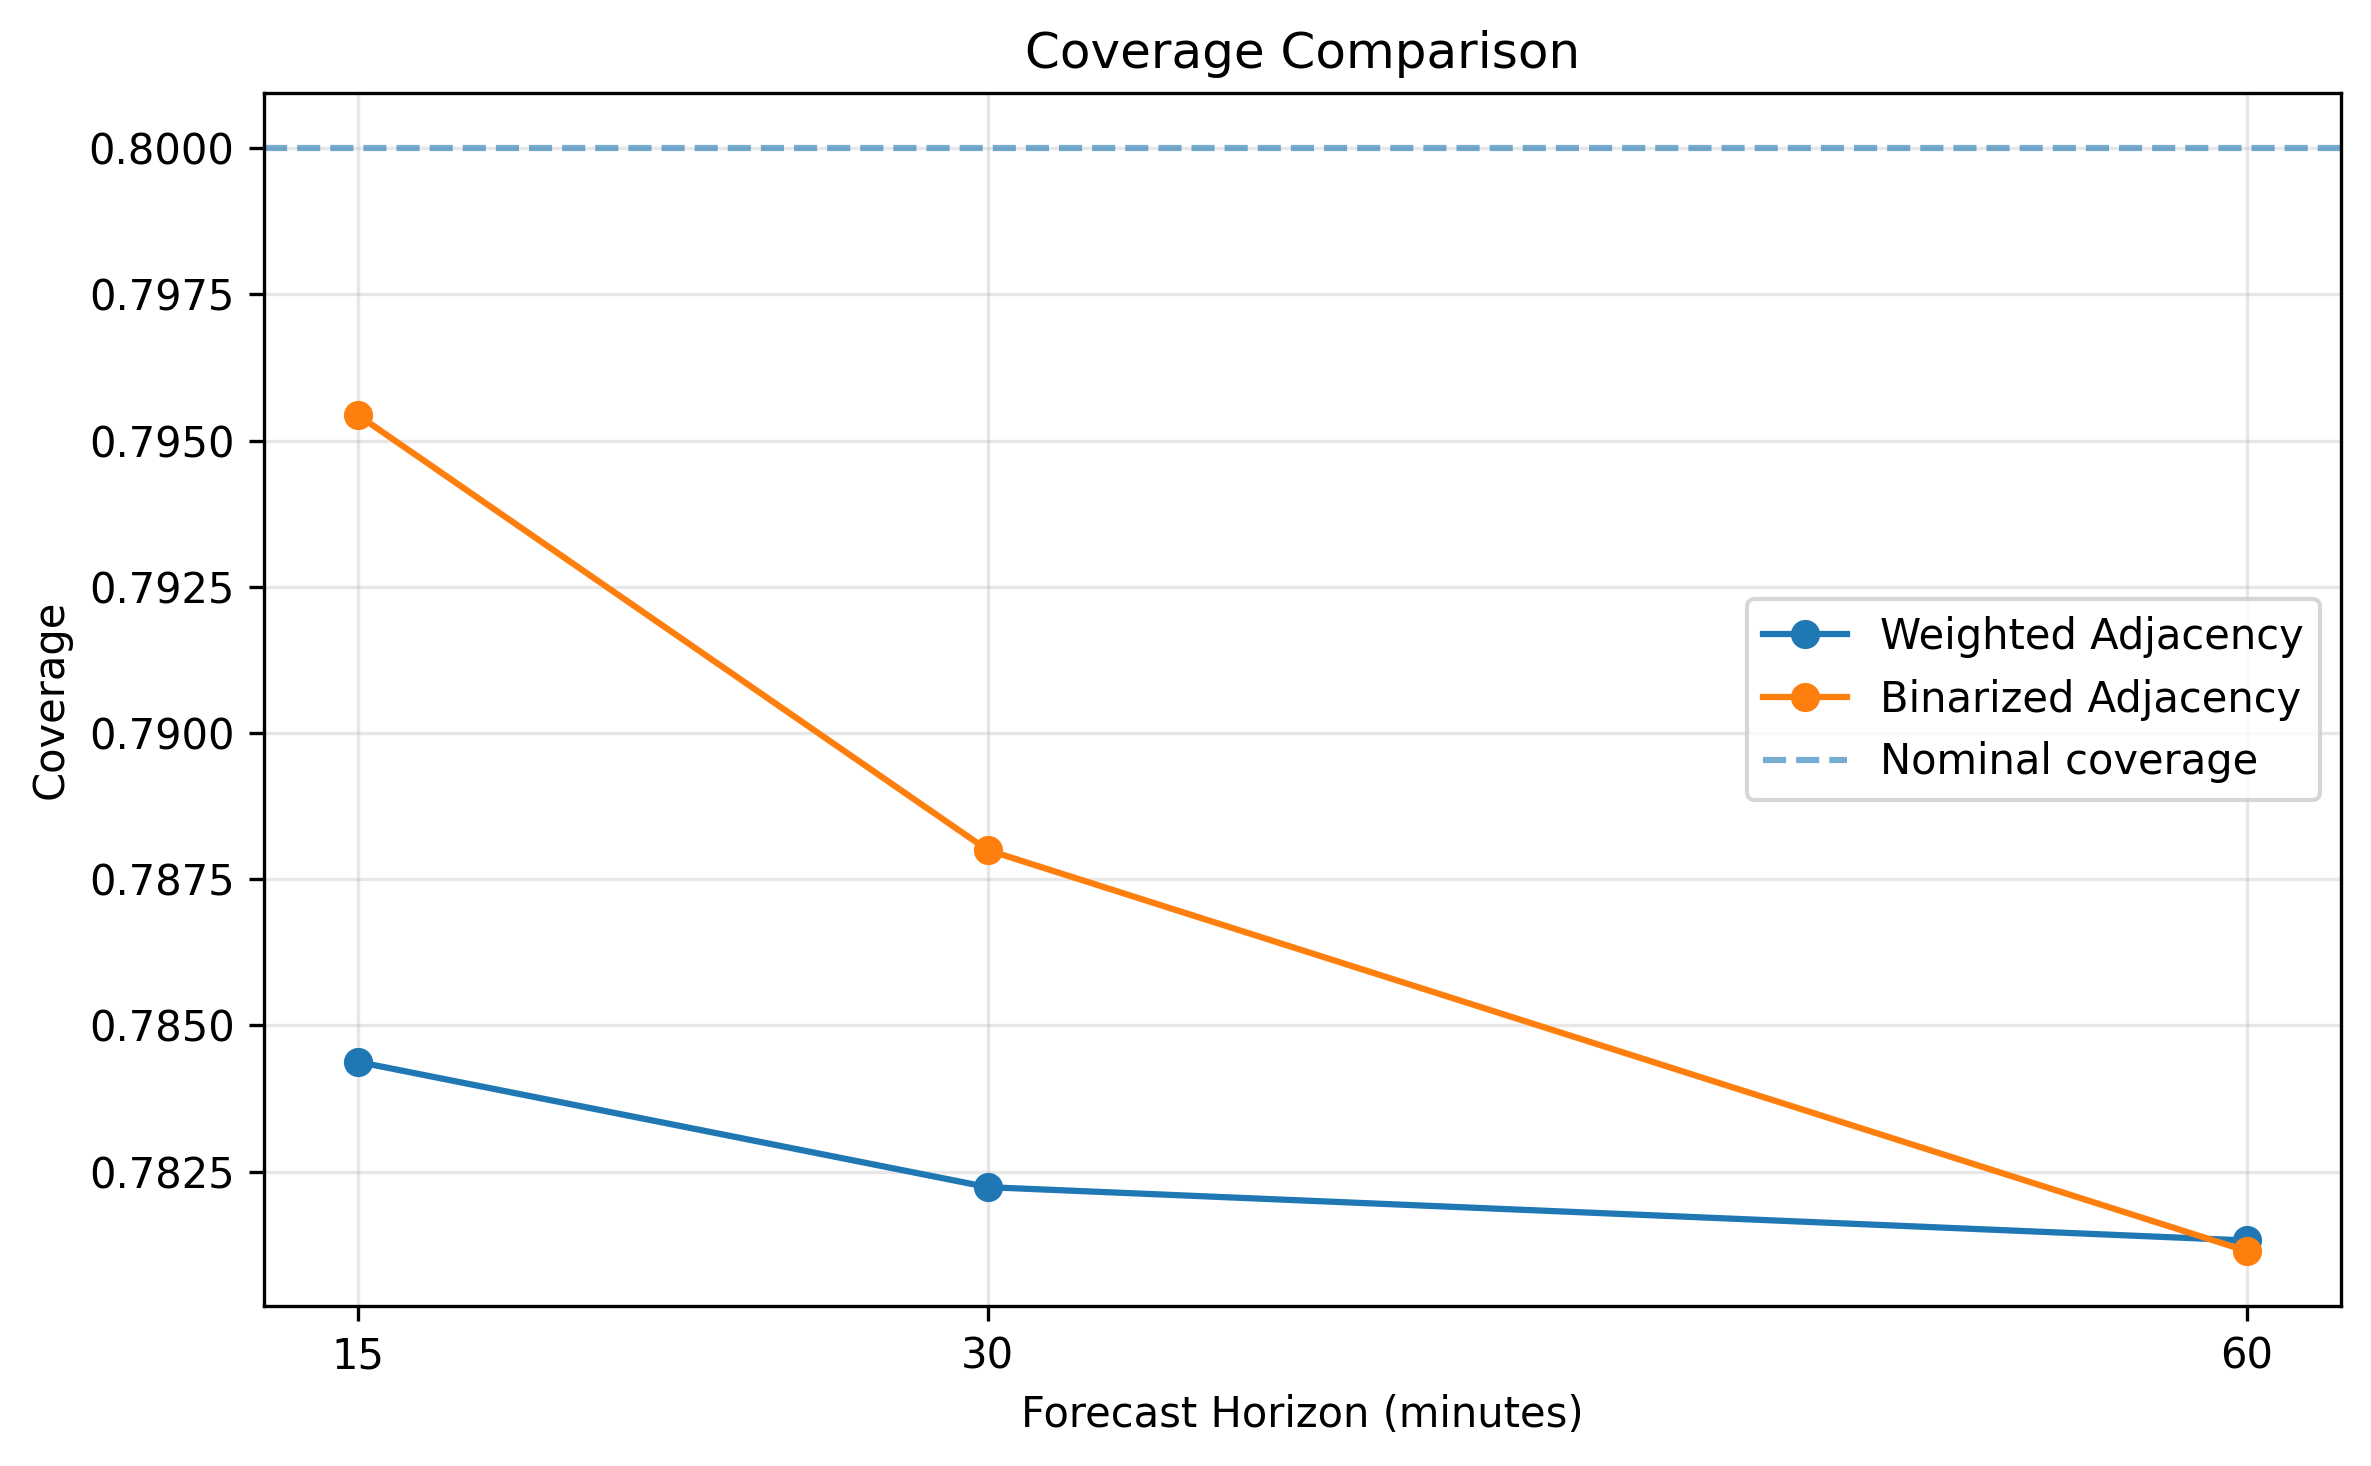
\includegraphics[width=\linewidth]{img/graph_temporal/ablation_comparison/coverage_graph_temporal_variant_comparison}
    \end{minipage}
    \hfill
    \begin{minipage}[b]{0.48\linewidth}
        \centering
        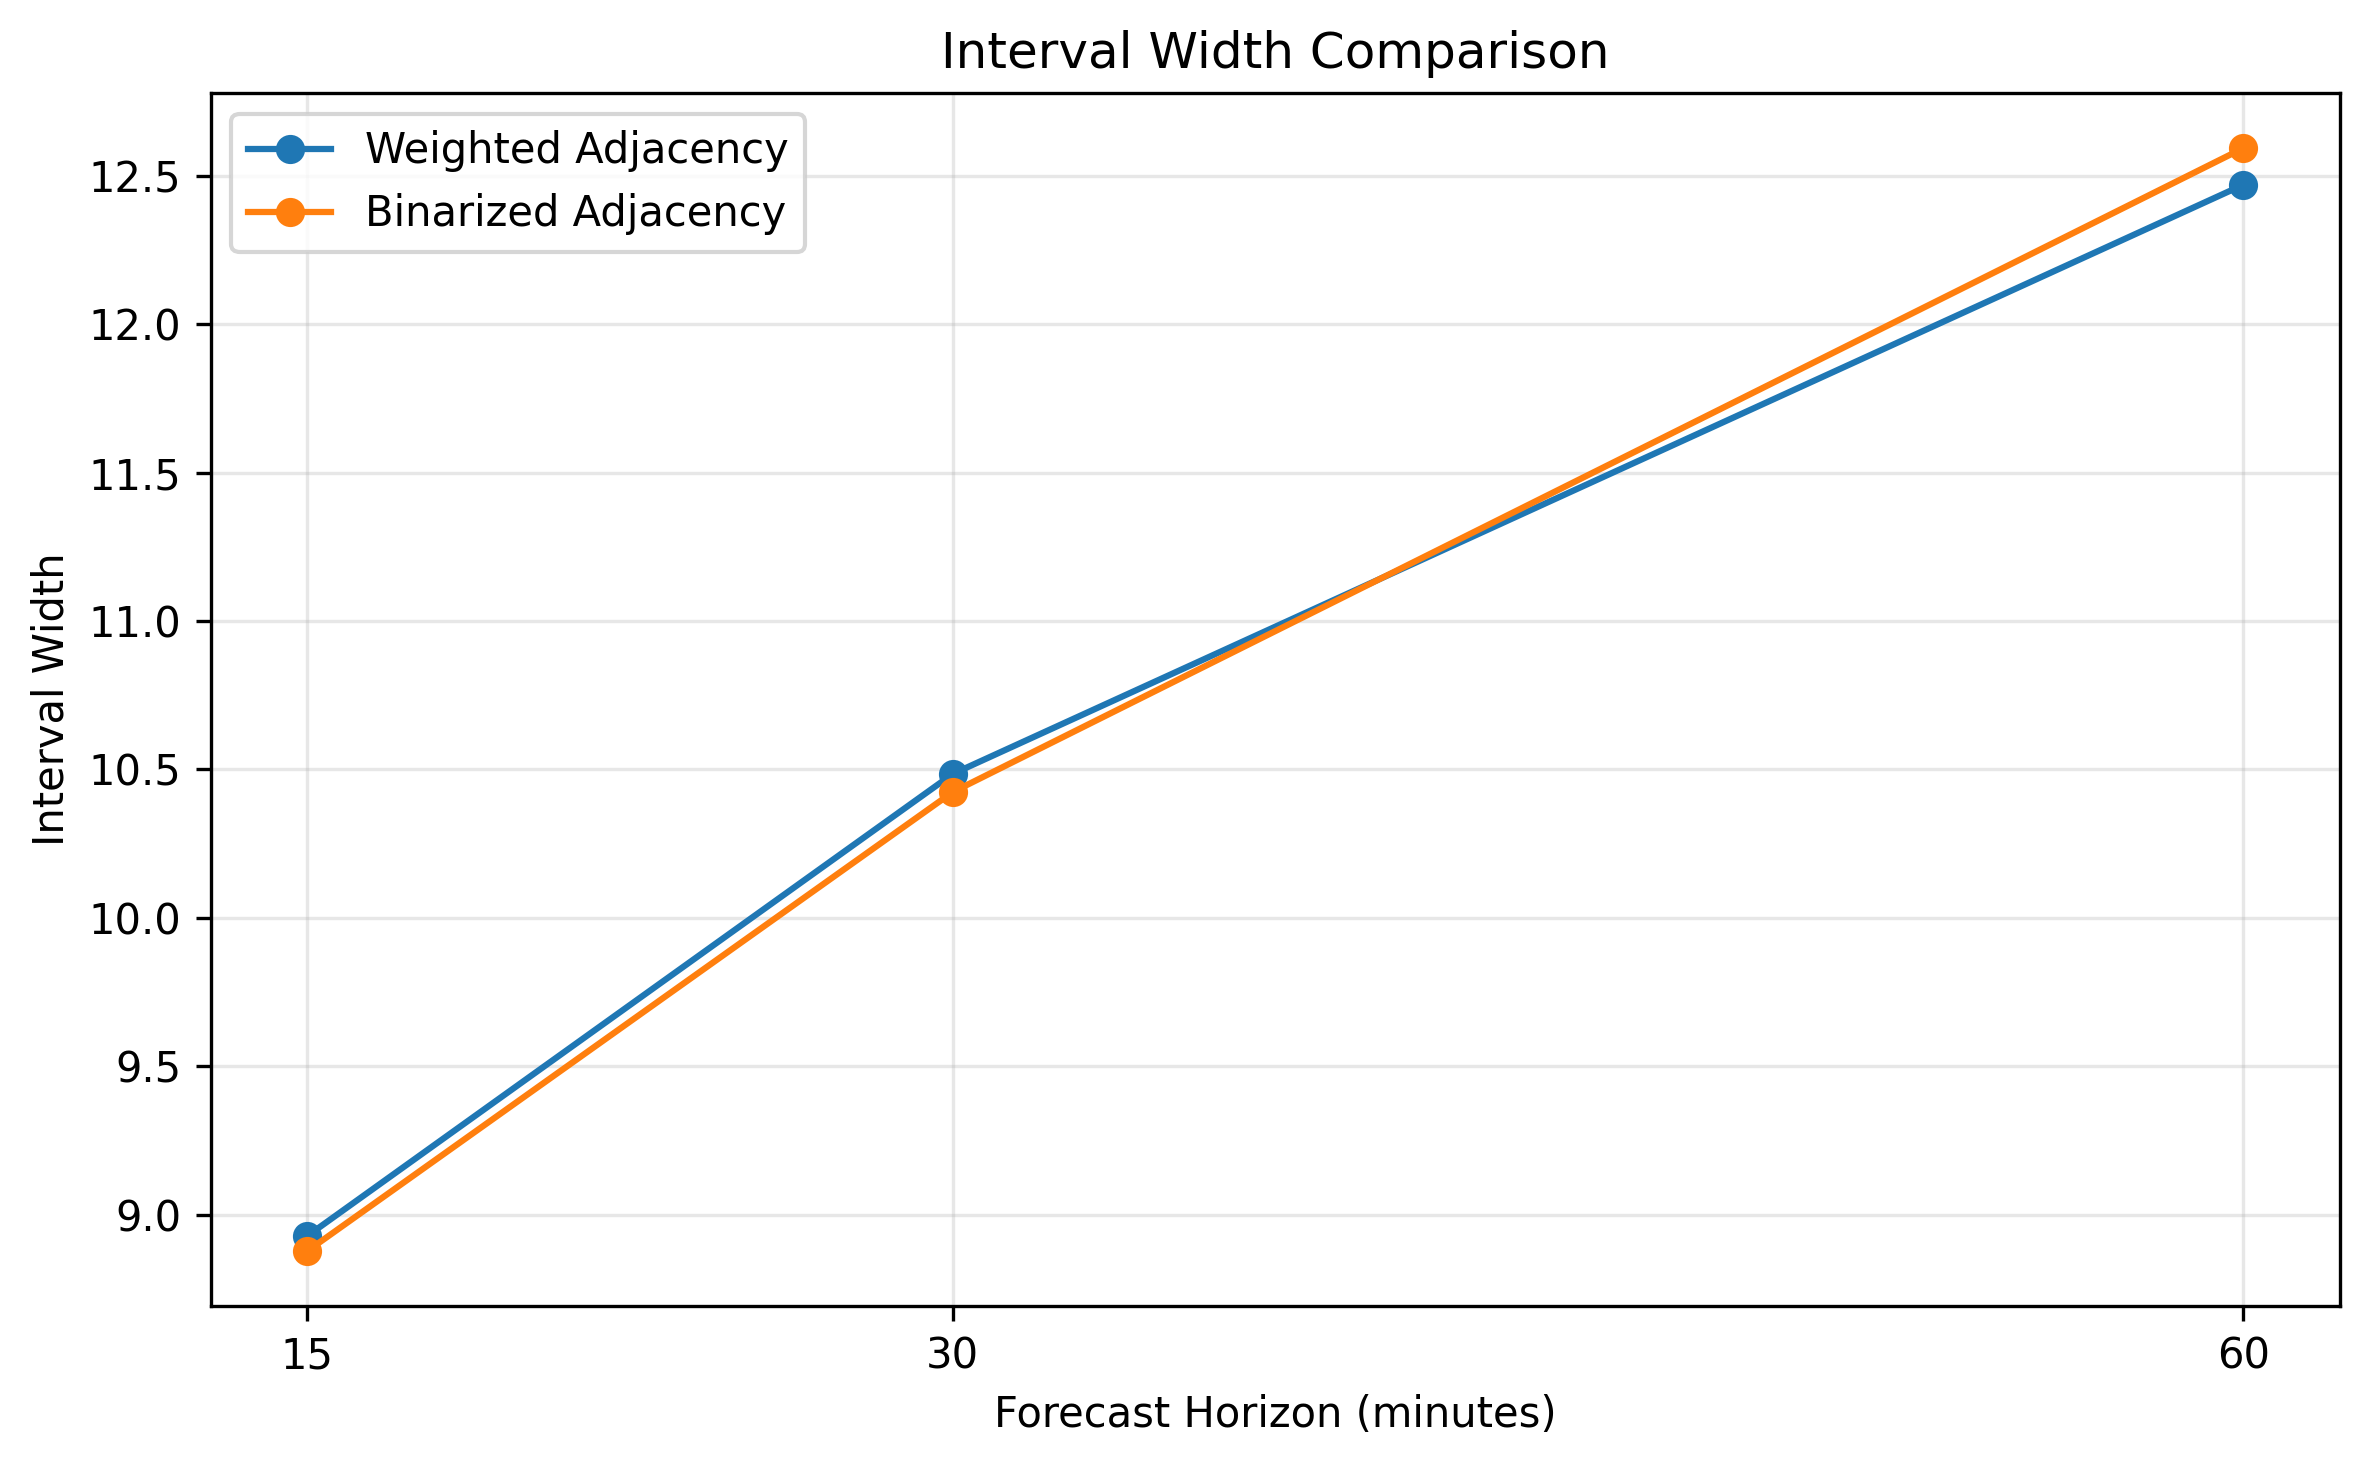
\includegraphics[width=\linewidth]{img/graph_temporal/ablation_comparison/interval_width_graph_temporal_variant_comparison}
    \end{minipage}

    \caption{Comparison of the Graph-Temporal model using the weighted and
    binary adjacency matrices. The top row reports point forecasting
    performance in terms of MAE (left) and RMSE (right), while the bottom
    row reports empirical coverage (left) and prediction interval width
    (right) across the three forecasting horizons.}
    \label{fig:weighted_binary_comparison}
\end{figure}

The comparison is further illustrated in
Figure~\ref{fig:weighted_binary_comparison}. The probabilistic results reveal
a more nuanced difference. At 15 and 30 minutes, the binary graph produces
slightly narrower intervals, while its empirical coverage is slightly closer
to the nominal 80\% level. At 60 minutes, however, the binary representation
produces a slightly wider interval, while coverage remains almost unchanged.
Therefore, binarizing the graph does not provide a consistent advantage in
terms of interval sharpness or reliability.


Overall, these results indicate that the benefit of graph message passing is
not determined solely by the presence of connections between sensors. The
relative edge weights provide useful information for spatial aggregation,
with their contribution becoming more evident as the forecasting horizon
increases. Since the binary graph does not provide a consistent improvement
in probabilistic reliability and results in higher point errors,
the original weighted adjacency matrix was retained for the main
Graph-Temporal model.